\setcounter{chapter}{10}
\chapter{Categorical Dependent Variables}
{\small \textit{Chapter Preview}. A model with a categorical
dependent variable allows one to predict whether an observation is a
member of a distinct group, or category. Binary variables represent
an important special case; they can indicate whether or not an event
of interest has occurred. In actuarial and financial applications,
the event may be whether a claim occurs, a person purchases
insurance, a person retires or a firm becomes insolvent. The chapter
introduces logistic regression and probit models of binary dependent
variables. Categorical variables may also represent more than two
groups, known as \emph{multicategory} outcomes. Multicategory
variables may be unordered or ordered, depending on whether it makes
sense to rank the variable outcomes. For unordered outcomes, known
as \emph{nominal} variables, the chapter introduces generalized
logits and multinomial logit models. For ordered outcomes, known as
\emph{ordinal} variables, the chapter introduces cumulative logit
and probit models.}

\section{Binary Dependent Variables}

We have already introduced binary variables as a special type of
discrete variable that can be used to indicate whether or not a
subject has a characteristic of interest, such as gender for a
person or ownership of a captive insurance company for a firm.
Binary variables also describe whether or not an event of interest
has occurred, such as an accident. A model with a binary dependent
variable allows one to predict whether an event has occurred or a
subject has a characteristic of interest.\index{categorical
variable!binary}

\linejed

\textbf{Example: MEPS Expenditures.}\ecaptionjed{MEPS Expenditures}
Section \ref{S11:MEPS} will describe an extensive database from the
Medical Expenditure Panel Survey (MEPS) on hospitalization
utilization and expenditures. For these data, we will consider
\begin{equation*}
y_i = \left\{
\begin{array}{ll}
1 & i\text{th person was hospitalized during the sample period} \\
0 & \text{otherwise}%
\end{array}%
\right. .
\end{equation*}%
There are $n=2,000$ persons in this sample, distributed as:
\vspace{-.2in}
 \scalefont{0.9}  \begin{center}  \begin{table}[h]
\caption{\label{T11:MEPSIntroStats} Hospitalization by Gender}
\begin{tabular}{ll|ll}
\hline
 &  &  Male & Female   \\ \hline
Not hospitalized & $y=0$ & 902 (95.3\%) & ~~941 (89.3\%)\\
Hospitalized & $y=1$ &  ~44 ( 4.7\%)  & ~~113 (10.7\%)\\
 Total &       & 946  & 1,054 \\
 \hline
\end{tabular}
\end{table}  \end{center}  \scalefont{1.1111}
\noindent Table \ref{T11:MEPSIntroStats} suggests that gender has an
important influence on whether someone becomes hospitalized.

\linejed
\bigskip

Like the linear regression techniques introduced in prior chapters, we are
interested in using characteristics of a person, such as their age, sex,
education, income and prior health status, to help explain the
dependent variable $y$. Unlike the prior chapters, now the dependent
variable is discrete and not even approximately normally distributed. In
limited circumstances, linear regression can be used with binary dependent
variables - this application is known as a \emph{linear probability model}.

\subsubsection*{Linear probability models}\index{regression model!linear
probability}\index{symbols!$\pi_i$, probability of a 1 for subject
$i$}

To introduce some of the complexities encountered with binary
dependent variables, denote the probability that the response equals
1 by $\pi_i= \mathrm{Pr}(y_i=1)$. A binary random
variable has a \emph{Bernoulli distribution}. Thus, we may interpret
the mean response as the probability that the response equals
one, that is, $\mathrm{E~}y_i=0\times \mathrm{Pr}(y_i=0) + 1 \times
\mathrm{Pr}(y_i=1) = \pi_i$. Further, the variance is related to the
mean through the expression $\mathrm{Var}~y_i = \pi_i(1-\pi_i)$.

\marginparjed{Linear probability models enjoy convenient parameter
interpretations.}

We begin by considering a linear model of the form%
\begin{equation*}
y_i = \mathbf{x}_i^{\mathbf{\prime}} \boldsymbol \beta +
\varepsilon_i,
\end{equation*}
known as a linear probability model. Assuming
$\mathrm{E~}\varepsilon_i=0$, we have that
$\mathrm{E~}y_i=\mathbf{x}_i^{\mathbf{\prime }} \boldsymbol \beta
=\pi_i$. Because $y_i$ has a Bernoulli distribution,
$\mathrm{Var}~y_i=\mathbf{x}_i^{\mathbf{\prime}} \boldsymbol
\beta(1-\mathbf{x}_i^{\mathbf{\prime}}\boldsymbol \beta)$. Linear
probability models are used because of the ease of parameter
interpretations. For large data sets, the computational simplicity
of ordinary least squares estimators is attractive when compared to
some complex alternative nonlinear models introduced later in this
chapter. As described in Chapter 3, ordinary least squares
estimators for $\boldsymbol \beta$ have desirable properties. It is
straightforward to check that the estimators are consistent and
asymptotically normal under mild conditions on the explanatory
variables \{$\mathbf{x}_i$\}. However, linear probability models
have several drawbacks that are serious for many applications.

\bigskip

\boxedjed

\textit{Drawbacks of the Linear Probability Model}

\begin{itemize}
\item \emph{Fitted values can be poor.} The expected response is a probability and thus must vary between 0
and 1. However, the linear combination,
$\mathbf{x}_i^{\mathbf{\prime}} \boldsymbol \beta$, can vary between
negative and positive infinity. This mismatch implies, for example,
that fitted values may be unreasonable.

\item \emph{Heteroscedasticity.} Linear models assume homoscedasticity (constant variance) yet the
variance of the response depends on the mean that varies over
observations. The problem of varying variability is known as
heteroscedasticity.\index{heteroscedasticity}

\item \emph{Residual analysis is meaningless.} The response must be either a 0 or 1 although the regression models
typically regards distribution of the error term as continuous. This
mismatch implies, for example, that the usual residual analysis in
regression modeling is meaningless.
\end{itemize}

\end{boxedminipage}
\bigskip

To handle the heteroscedasticity problem, a (two-stage) weighted
least squares procedure is possible. In the first stage,
one uses ordinary least squares to compute estimates of $\boldsymbol
\beta$. With this estimate, an estimated variance for each subject
can be computed using the
relation $\mathrm{Var}~y_i=\mathbf{x}_i^{\mathbf{\prime}}\boldsymbol \beta%
(1-\mathbf{x}_i^{\mathbf{\prime}}\boldsymbol \beta)$. At the second
stage, a weighted least squares is performed using the inverse of
the estimated variances as weights to arrive at new estimates of
$\boldsymbol \beta$. It is possible to iterate this procedure,
although studies have shown that there are few advantages in doing
so (see Carroll and Ruppert, 1988). Alternatively, one can use
ordinary least squares estimators of $\boldsymbol \beta$ with
standard errors that are robust to heteroscedasticity (see Section
5.7.2).\index{heteroscedasticity-consistent standard error}

\section{Logistic and Probit Regression
Models}\label{S11:LogProbModels}\index{regression
model!logistic}\index{regression
model!probit}\index{symbols!$\mathrm{\pi}(\cdot)$, probability
function}

\subsection{Using Nonlinear Functions of Explanatory Variables}

To circumvent the drawbacks of linear probability models, we consider
alternative models in which we express the expectation of the response as a
function of explanatory variables, $\pi_i=\mathrm{\pi }(\mathbf{x}_i^{%
\mathbf{\prime}}\boldsymbol \beta)=\Pr (y_i=1|\mathbf{x}_i)$. We
focus on two special cases of the function $\mathrm{\pi
}(\cdot)$:

\begin{itemize}
\item $\mathrm{\pi }(z)=\frac{1}{1+\exp (-z)}=\frac{e^{z}}{1+e^{z}}$, the
logit case, and

\item $\mathrm{\pi }(z)=\mathrm{\Phi }(z)$, the probit case.
\end{itemize}

\noindent Here, $\mathrm{\Phi }(\cdot)$ is the standard normal
distribution function. The choice of the identity function (a
special kind of linear function), $\mathrm{\pi }(z)=z$, yields the
linear probability model. In contrast, $\mathrm{\pi}$ is nonlinear
for both the logit and probit cases. These two functions are similar
in that they are almost linearly related over the interval $0.1\leq
p\leq 0.9$. Thus, to a large extent, the function choice is
dependent on the preferences of the analyst. Figure
\ref{F11:LogitProbit} compares the logit and probit functions
showing that it will be difficult to distinguish between the two
specifications with most data sets.


The inverse of the function, $\mathrm{\pi }^{-1}$, specifies the
form of the probability that is linear in the explanatory variables,
that is, $\mathrm{\pi }^{-1}(\pi_i)=
\mathbf{x}_i^{\mathbf{\prime}}\boldsymbol \beta$. In Chapter 13, we
refer to this inverse as the \emph{link function}.\index{link
function}


\begin{figure}[htp]
  \begin{center}
    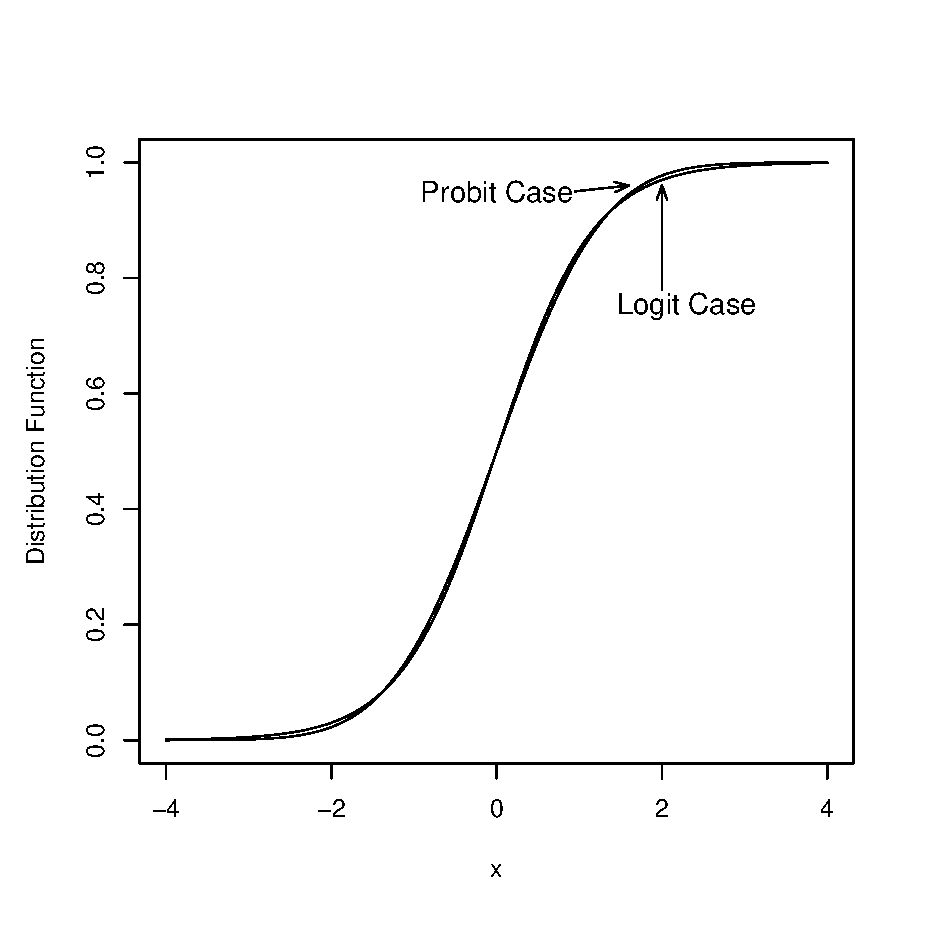
\includegraphics[width=1\textwidth,angle=0,scale=0.5]{Chapter11Binary/F11LogitProbit.eps}
    \caption{\label{F11:LogitProbit} \small Comparison of Logit and Probit (Standard Normal) Distribution
Functions}
  \end{center}
\end{figure}


\linejed\index{actuarial \& financial terms and concepts!credit
scoring}\index{examples!credit scores}

\textbf{Example: Credit Scoring.}\ecaptionjed{Credit Scoring} Banks,
credit bureaus and other financial institutions develop ``credit
scores'' for individuals that are used to predict the likelihood
that the borrower will repay current and future debts. Individuals who
do not meet stipulated repayment schedules in a loan agreement are
said to be in ``default.'' A credit score is then a predicted
probability of being in default, with the credit application
providing the explanatory variables used in developing the credit
score. The choice of explanatory variables depends on the purpose of
the application; credit scoring is used for issuing credit cards for
making small consumer purchases as well as mortgage applications for
multimillion dollar houses. In Table
\ref{T11:CreditCharacteristics}, Hand and Henley (1997) provide a
list of typical characteristics that are used in credit scoring.


\scalefont{0.9}
\begin{table}[h]
\caption{\label{T11:CreditCharacteristics} Characteristics Used in
Some Credit Scoring Procedures}
\begin{tabular}{ll}
   \hline
Characteristics & Potential Values \\
\hline Time at present address & 0-1, 1-2, 3-4, 5+ years \\
Home status & Owner, tenant, other \\
Postal Code & Band A, B, C, D, E \\
Telephone & Yes, no \\
Applicant's annual income & \pounds (0-10000), \pounds
(10,000-20,000)
\pounds(20,000+) \\
Credit card & Yes, no \\
Type of bank account & Check and/or savings, none \\
Age & 18-25, 26-40, 41-55, 55+ years \\
County Court judgements & Number \\
Type of occupation & Coded \\
Purpose of loan & Coded \\
Marital status & Married, divorced, single, widow, other \\
Time with bank & Years \\
Time with employer & Years \\
 \hline
     \multicolumn{2}{c}{\textit{Source}: Hand and Henley (1997)} \\
\end{tabular}
\end{table}
\scalefont{1.1111}

\bigskip

With credit application information and default experience, a
logistic regression model can be used to fit the probability of
default with credit scores resulting from fitted values. Wiginton
(1980) provides an early application of logistic regression to
consumer credit scoring. At that time, other statistical methods
known as discriminant analysis were at the cutting edge of
quantitative scoring methodologies. In their review article, Hand
and Henley (1997) discuss other competitors to logistic regression
including machine learning systems and neural networks. As noted by
Hand and Henley, there is no uniformly ``best'' method. Regression
techniques are important in their own right due to their widespread
usage and because they can provide a platform for learning about
newer methods.

\marginparjed{Regression techniques are important due to their
widespread usage and because they can provide a platform for
learning about newer methods.}

Credit scores provide estimates of the likelihood of defaulting on
loans but issuers of credit are also interested in the amount and
timing of debt repayment. For example, a ``good'' risk may repay a
credit balance so promptly that little profit is earned by the
lender. Further, a ``poor'' mortgage risk may default on a loan so
late in the duration of the contract that a sufficient profit was
earned by the lender. See Gourieroux and Jasiak (2007) for a broad
discussion of how credit modeling can be used to assess the
riskiness and profitability of loans.

\linejed

\subsection{Threshold Interpretation}\label{S11:Threshold}
\index{symbols!$y^{\ast}$, unobserved latent variable}

Both the logit and probit cases can be interpreted as follows.
Suppose that there exists an \emph{underlying} linear model,
$y_i^{\ast} = \mathbf{x}_i^{\mathbf{\prime}}\boldsymbol \beta
 + \varepsilon_i^{\ast}$. Here, we do not observe the response
$y_i^{\ast}$ yet interpret it to be the ``propensity'' to possess a
characteristic. For example, we might think about the financial
strength of an insurance company as a measure of its propensity to
become insolvent (no longer capable of meeting its financial
obligations). Under the threshold interpretation, we do not observe
the propensity but we do observe when the propensity crosses a
threshold. It is customary to assume that this threshold is 0, for
simplicity. Thus, we observe
\begin{equation*}
y_i=\left\{
\begin{array}{ll}
0 & y_i^{\ast}\leq 0 \\
1 & y_i^{\ast}>0
\end{array}
\right. .
\end{equation*}

\index{distributions!logistic}

To see how the logit case is derived from the threshold model,
assume a logistic distribution function for the disturbances, so that
\begin{equation*}
\mathrm{\Pr }(\varepsilon_i^{\ast}\leq a)=\frac{1}{1+\exp (-a)}.
\end{equation*}
Like the normal distribution, one can verify by calculating the density that the logistic distribution
is symmetric about zero. Thus, $-\varepsilon_i^{\ast}$ has the same distribution as $\varepsilon_i^{\ast}$ and so
\begin{equation*}
\pi_i=\Pr (y_i=1|\mathbf{x}_i)=\mathrm{\Pr }(y_i^{\ast}>0)=\mathrm{%
\Pr }(\varepsilon_i^{\ast}\leq \mathbf{x}_i^{\mathbf{\prime}}\mathbf{%
\beta })=\frac{1}{1+\exp (-\mathbf{x}_i^{\mathbf{\prime}}\boldsymbol \beta)}%
=\mathrm{\pi }(\mathbf{x}_i^{\mathbf{\prime}}\boldsymbol \beta).
\end{equation*}
This establishes the threshold interpretation for the logit case.
The development for the probit case is similar and is omitted.

\subsection{Random Utility Interpretation}\index{utility function}

Both the logit and probit cases are also justified by appealing
to the following ``random utility'' interpretation of the model. In
some economic applications, individuals select one of two choices.
Here, preferences among choices are indexed by an unobserved utility
function; individuals select the choice that provides the greater
utility.

For the $i$th subject, we use the notation $u_i$ for this utility function.
We model the utility ($U$) as a function of an underlying value ($V$) plus random
noise ($\varepsilon$), that is, $U_{ij}=u_i(V_{ij}+\varepsilon_{ij})$, where $j$ may
be 1 or 2, corresponding to the choice. To illustrate, we assume
that the individual chooses the category corresponding to $j=1$ if
$U_{i1}>U_{i2}$ and denote this choice as $y_i=1$. Assuming that
$u_i$ is a strictly increasing function, we have
\begin{eqnarray*}
\Pr (y_i &=&1)=\mathrm{\Pr }(U_{i2}<U_{i1})=\mathrm{\Pr }\left(
u_i(V_{i2}+\varepsilon_{i2})<u_i(V_{i1}+\varepsilon_{i1})\right) \\
&=&\mathrm{\Pr }(\varepsilon_{i2}-\varepsilon_{i1}<V_{i1}-V_{i2}).
\end{eqnarray*}

To parameterize the problem, assume that the value $V$ is an unknown
linear combination of explanatory variables. Specifically, we take
$V_{i2}=0$ and $V_{i1}=\mathbf{x}_i^{\mathbf{\prime}}\boldsymbol
\beta$. We may take the difference in the errors,
$\varepsilon_{i2}-\varepsilon_{i1}$, as normal or logistic,
corresponding to the probit and logit cases, respectively. The
logistic distribution is satisfied if the errors are assumed to have
an \emph{extreme-value}, or \emph{Gumbel}, distribution (see, for
example, Amemiya, 1985).\index{distributions!extreme
value}\index{symbols!$V$, underlying value}\index{symbols!$U$,
utility}

\subsection{Logistic Regression}\label{S11:LogisticRegression}

An advantage of the logit case is that it permits closed-form expressions,
unlike the normal distribution function. \emph{Logistic regression} is
another phrase used to describe the logit case.

Using $p=\mathrm{\pi }(z)= \left( 1+ \mathrm{e}^{-z}\right)^{-1}$,
the inverse of $\mathrm{\pi }$ is calculated as $z=\mathrm{\pi
}^{-1}(p)=\ln(p/(1-p))$. To simplify future presentations, we define
\begin{equation*}
\mathrm{logit}(p)=\ln \left( \frac{p}{1-p}\right)
\end{equation*}
to be the \emph{logit function}. With a logistic regression model,
we represent the linear combination of explanatory variables as the
logit of the success probability, that is,
$\mathbf{x}_i^{\mathbf{\prime}}\boldsymbol \beta
=\mathrm{logit}(\pi_i)$.\index{logit function}

\subsubsection*{Odds interpretation}\index{odds}

When the response $y$ is binary, knowing only $p=\Pr(y=1)$
summarizes the entire distribution. In some applications, a simple
transformation of $p$ has an important interpretation. The lead
example of this is the \emph{odds}, given by $p/(1-p)$. For example,
suppose that $y$ indicates whether or not a horse wins a race and
$p$ is the probability of
the horse winning. If $p=0.25$, then the odds of the horse winning is $%
0.25/(1.00-0.25)=0.3333$. We might say that the odds of winning are 0.3333
to 1, or one to three. Equivalently, we say that the probability of not
winning is $1-p=0.75$ so that the odds of the horse not winning is $%
0.75/(1-0.75)=3$ and the odds against the horse are three to one.

Odds have a useful interpretation from a betting standpoint. Suppose that we
are playing a fair game and that we place a bet of \$1 with one to three
odds. If the horse wins, then we get our \$1 back plus winnings of \$3. If
the horse loses, then we lose our bet of \$1. It is a fair game in the sense
that the expected value of the game is zero because we win \$3 with
probability $p=0.25$ and lose \$1 with probability $1-p=0.75$. From an
economic standpoint, the odds provide the important numbers (bet of \$1 and
winnings of \$3), not the probabilities. Of course, if we know $p$, then we
can always calculate the odds. Similarly, if we know the odds, we can always
calculate the probability $p$.

The logit is the logarithmic odds function, also known as the
\emph{log odds}.\index{log odds}

\subsubsection*{Odds ratio interpretation}

To interpret the regression coefficients in the logistic regression model, $%
\boldsymbol \beta=(\beta_0,\ldots ,\beta_{k})^{\prime}$, we begin by
assuming that $j$th explanatory variable, $x_{ij}$, is either 0 or
1. Then, with the notation $\mathbf{x}_i=(x_{i0},...,x_{ij},\ldots
,x_{ik})^{\prime}$, we may interpret

\begin{eqnarray*}
\beta_j &=&(x_{i0},...,1,\ldots ,x_{ik})^{\prime}\boldsymbol \beta%
-(x_{i0},...,0,\ldots ,x_{ik})^{\prime}\boldsymbol \beta \\
&=&\ln \left( \frac{\Pr (y_i=1|x_{ij}=1)}{1-\Pr
(y_i=1|x_{ij}=1)}\right) -\ln \left( \frac{\Pr
(y_i=1|x_{ij}=0)}{1-\Pr (y_i=1|x_{ij}=0)}\right)
\end{eqnarray*}

Thus,

\begin{equation*}
e^{\beta_j}=\frac{\Pr (y_i=1|x_{ij}=1)/\left( 1-\Pr
(y_i=1|x_{ij}=1)\right) }{\Pr (y_i=1|x_{ij}=0)/\left( 1-\Pr
(y_i=1|x_{ij}=0)\right) }.
\end{equation*}\index{odds ratio}
This shows that $e^{\beta_j}$ can be expressed as the ratio of two
odds, known as the \emph{odds ratio}. That is, the numerator of this
expression is the odds when $x_{ij}=1,$ whereas the denominator is
the odds when $x_{ij}=0$. Thus, we can say that the odds when
$x_{ij}=1$ are $\exp (\beta_j)$ times as large as the odds when
$x_{ij}=0$. To illustrate, suppose $\beta_j=0.693$, so that $\exp
(\beta _j)=2$. From this, we say that the odds (for $y=1$) are twice
as great for $x_{ij}=1$ as for $x_{ij}=0$.

Similarly, assuming that $j$th explanatory variable is continuous
(differentiable), we have
\begin{eqnarray}\label{E11:OddsRatioElasticity}
\beta_j &=&\frac{\partial }{\partial x_{ij}}\mathbf{x}_i^{\prime}
\boldsymbol \beta =\frac{\partial }{\partial x_{ij}}\ln \left(
\frac{\Pr (y_i=1|x_{ij})}{1-\Pr (y_i=1|x_{ij})}\right)   \nonumber \\
&=&\frac{\frac{\partial }{\partial x_{ij}}\Pr (y_i=1|x_{ij})/\left(
1-\Pr (y_i=1|x_{ij})\right) }{\Pr (y_i=1|x_{ij})/\left( 1-\Pr
(y_i=1|x_{ij})\right) }.
\end{eqnarray}
Thus, we may interpret $\beta_j$ as the proportional change in the
odds ratio, known as an \emph{elasticity} in
economics.\index{actuarial \& financial terms and
concepts!elasticity}

\marginparjed{We may interpret $\beta_j$ as the proportional change
in the odds ratio.}

\linejed

\textbf{Example: MEPS Expenditures - Continued.} Table
\ref{T11:MEPSIntroStats} shows that the percentage of females who
were hospitalized is $10.7\%$; alternatively, the odds of females
being hospitalized is $0.107/(1-0.107)=0.120$. For males, the
percentage is $4.7\%$ so that the odds were $0.0493$. The odds ratio
is $0.120/0.0493=2.434$; females are more than twice as likely to be
hospitalized as males.

From a logistic regression fit (described in Section
\ref{S11:MEPS}), the coefficient associated with gender is $0.733$.
Based on this model, we say that females are $\exp
(0.733)=2.081$ times as likely as males to be hospitalized. The
regression estimate of the odds ratio controls for additional
variables (such as age and education) compared to the
basic calculation based on raw frequencies.


\linejed

\section{Inference for Logistic and Probit Regression Models}

\subsection{Parameter Estimation}

The customary method of estimation for logistic and probit models is
\emph{maximum likelihood}, described in further detail in Section
\ref{S11:LikelihoodInference}. To provide intuition, we outline the
ideas in the context of binary dependent variable regression models.

\index{likelihood inference!maximum likelihood
estimator}\index{likelihood inference!likelihood}\index{likelihood
inference!log-likelihood}

The \emph{likelihood }is the observed value of the probability
function. For a single observation, the likelihood is
\begin{equation*}
\left\{
\begin{array}{ll}
1-\pi_i & \mathrm{if}\ y_i=0 \\
\pi_i & \mathrm{if}\ y_i=1
\end{array}
\right. .
\end{equation*}\index{estimator!maximum likelihood}
The objective of maximum likelihood estimation is to find the
parameter values that produce the largest likelihood. Finding the
maximum of the logarithmic function yields the same solution as
finding the maximum of the corresponding function. Because it is
generally computationally simpler, we consider the logarithmic (or
log-) likelihood, written as
\begin{equation}\label{E11:LogLikBin}
\left\{
\begin{array}{ll}
\ln \left( 1-\pi_i\right) & \mathrm{if}\ y_i=0 \\
\ln \pi_i & \mathrm{if}\ y_i=1
\end{array}
\right. .
\end{equation}
More compactly, the log-likelihood of a single observation is
\begin{equation*}
y_i\ln \mathrm{\pi }(\mathbf{x}_i^{\mathbf{\prime}}\boldsymbol
\beta) + (1-y_i) \ln \left( 1-\mathrm{\pi }(\mathbf{x}_i^{\mathbf{\prime}}%
\boldsymbol \beta)\right) ,
\end{equation*}
where $\pi_i=\mathrm{\pi }(\mathbf{x}_i^{\mathbf{\prime}}\boldsymbol \beta%
). $ Assuming independence among observations, the likelihood of the data
set is a product of likelihoods of each observation. Taking logarithms, the
log-likelihood of the data set is the sum of log-likelihoods of single
observations.

\marginparjed{The log-likelihood is viewed as a function of the
parameters, with the data held fixed. In contrast, the joint
probability mass function is viewed as a function of the realized
data, with the parameters held fixed.}


\bigskip

\boxedjed\index{goodness of fit statistics!log-likelihood}

The log-likelihood of the data set is
\begin{equation}\label{E11:LogLike}
L(\boldsymbol \beta)=\sum\limits_{i=1}^{n}\left\{ y_i\ln \mathrm{\pi
}( \mathbf{x}_i^{\mathbf{\prime}}\boldsymbol \beta) + (1-y_i) \ln
\left( 1- \mathrm{\pi }(\mathbf{x}_i^{\mathbf{\prime}}\boldsymbol
\beta)\right) \right\} .
\end{equation}
The log-likelihood is viewed as a function of the parameters, with
the data held fixed. In contrast, the joint probability mass
function is viewed as a function of the realized data, with the
parameters held fixed.

\end{boxedminipage}
\bigskip

The \emph{method of maximum likelihood} involves finding the values
of $\boldsymbol \beta$ that maximize the log-likelihood. The
customary method of finding the maximum is taking partial
derivatives with respect to the parameters of interest and finding
roots of the resulting equations. In this case, taking partial
derivatives with respect to $\boldsymbol \beta$ yields the
\emph{score equations}\index{likelihood inference!score equations}

\begin{equation} \label{E11:Score}
\frac{\partial }{\partial \boldsymbol \beta}L(\boldsymbol \beta%
)=\sum\limits_{i=1}^{n}\mathbf{x}_i\left( y_i-\mathrm{\pi
}(\mathbf{x}_i^{\mathbf{\prime}}\boldsymbol \beta)\right)
\frac{\mathrm{\pi }^{\prime}(
\mathbf{x}_i^{\mathbf{\prime}}\boldsymbol \beta)}{\mathrm{\pi
}(\mathbf{x}_i^{\mathbf{\prime}}\boldsymbol \beta)(1-\mathrm{\pi
}(\mathbf{x}_i^{ \mathbf{\prime}}\boldsymbol \beta))}=\mathbf{0},
\end{equation}
where $\pi^{\prime}$ is the derivative of $\pi$. The solution of these equations, denoted as $\mathbf{b}_{MLE}$, is
the maximum likelihood estimator. For the logit
function the score equations reduce to

\begin{equation}\label{E11:LogitScore}
\frac{\partial }{\partial \boldsymbol \beta}L(\boldsymbol \beta
)=\sum\limits_{i=1}^{n}\mathbf{x}_i\left( y_i-\mathrm{\pi }(\mathbf{x}
_i^{\mathbf{\prime}}\boldsymbol \beta)\right) =\mathbf{0},
\end{equation}
where $\mathrm{\pi }(z)=1/(1+\exp (-z))$.
\index{symbols!$\mathbf{b}_{MLE}$, maximum likelihood estimator of
$\boldsymbol \beta$}

\subsection{Additional Inference}

An estimator of the large sample variance of $\boldsymbol \beta$ may
be calculated taking partial derivatives of the score equations.
Specifically, the term\index{likelihood inference!information
matrix}
\begin{equation*}
\mathbf{I}(\boldsymbol \beta) = - \mathrm{E} \left( \frac{\partial^2}
{\partial \boldsymbol \beta ~ \partial \boldsymbol \beta
^{\prime}}L(\boldsymbol \beta) \right)
\end{equation*}
is the \emph{information matrix}. As a special case, using the logit
function and equation (\ref{E11:LogitScore}), straightforward
calculations show that the information matrix is
\begin{equation*}
\mathbf{I}(\boldsymbol \beta) = \sum\limits_{i=1}^{n} \sigma_i^2
\mathbf{x}_i \mathbf{x}_i^{\prime}
\end{equation*}
where $\sigma_i^2 = \mathrm{\pi} (\mathbf{x}_i^{\prime} \boldsymbol
\beta) (1 - \mathrm{\pi}(\mathbf{x}_i^{\prime} \boldsymbol \beta))$.
The square root of the $(j+1)st$ diagonal element of this matrix
evaluated at $\boldsymbol \beta = \mathbf{b}_{MLE}$ yields the
standard error for $b_{j,MLE}$, denoted as $se(b_{j,MLE})$.

To assess the overall model fit, it is customary to cite
\emph{likelihood ratio test statistics} in nonlinear regression
models. To test the overall model adequacy $H_0:\boldsymbol
\beta=\mathbf{0}$, we use the statistic\index{hypothesis test!test
statistics!likelihood ratio}\index{symbols!$LRT$, likelihood ratio
test statistic}

\begin{equation*}
LRT=2\times (L(\mathbf{b}_{MLE})-L_0),
\end{equation*}
where $L_0$ is the maximized log-likelihood with only an intercept
term. Under the null hypothesis $H_0$, this statistic has a
chi-square distribution with $k$ degrees of freedom. Section
\ref{S11:HypTests} describes likelihood ratio test statistics in
greater technical detail.\index{distributions!chi-square}

As described in Section \ref{S11:LikelihoodInference}, measures of
goodness of fit can be difficult to interpret in nonlinear models.
One measure is the so-called $max-scaled~R^2$, defined as
$R_{ms}^2=R^2/R_{max}^2$, where
\begin{equation*}
R^2=1-\left( \frac{\exp (L_0/n)}{\exp
(L(\mathbf{b}_{MLE})/n)}\right)
\end{equation*}
and $R_{max }^2 = 1 - \exp(L_0/n)^2$. Here, $L_0/n$ represents the
average value of this log-likelihood.\index{goodness of fit
statistics!max-scaled $R^2$}\index{goodness of fit
statistics!pseudo-$R^2$}

Another measure is a ``\emph{pseudo-}$R^2$''
\begin{equation*}
\frac{L( \mathbf{b}_{MLE}) - L_0}{L_{max}-L_0},
\end{equation*}
where $L_0$\ and $L_{max }$\ is the log-likelihood based on only an
intercept and on the maximum achievable, respectively. Like the
coefficient of determination, the pseudo-$R^2$ takes on values
between zero and one, with larger values indicating a better fit to
the data. Other versions of pseudo-$R^2$'s are available in the
literature, see, for example, Cameron and Trivedi (1998). An
advantage of this pseudo-$R^2$ measure is its link to hypothesis
testing of regression coefficients.


\linejed\index{examples!job security}

\textbf{Example: Job Security.}\ecaptionjed{Job Security} Valletta
(1999) studied declining job security using the Panel Survey of
Income Dynamics (PSID) database. We consider here one of the
regression models presented by Valletta, based on a sample of male
heads of households that consists of $n=24,168$ observations over the
years 1976-1992, inclusive. The PSID survey records reasons why men
left their most recent employment, including plant closures,
\textquotedblleft quit\textquotedblright\ and changed jobs for other
reasons. However, Valletta focused on dismissals (``laid off'' or
``fired'') because involuntary separations are associated with job
insecurity.

Table \ref{T11:DismissalProbs} presents a probit regression model
run by Valletta (1999), using dismissals as the dependent variable.
In addition to the explanatory variables listed in Table
\ref{T11:DismissalProbs}, other variables controlled for consisted
of education, marital status, number of children, race, years of
full-time work experience and its square, union membership,
government employment, logarithmic wage, the U.S. employment rate
and location as measured through the Metropolitan Statistical Area
residence. In Table \ref{T11:DismissalProbs}, tenure is years
employed at the current firm. Further, sector employment was
measured by examining the Consumer Price Survey employment in 387
sectors of the economy, based on 43 industry categories and nine
regions of the country.

On the one hand, the tenure coefficient reveals that more
experienced workers are less likely to be dismissed. On the other
hand, the coefficient associated with the interaction between tenure
and time trend reveals an increasing dismissal rate for experienced
workers.

The interpretation of the sector employment coefficients is also of
interest. With an average tenure of about 7.8 years in the sample,
we see the low tenure men are relatively unaffected by changes in
sector employment. However, for more experienced men, there is an
increasing probability of dismissal associated with sectors of the
economy where growth declines.\bigskip

\scalefont{0.9}
\begin{table}[h]
\caption{\label{T11:DismissalProbs} Dismissal Probit Regression
Estimates}
\begin{center}
\begin{tabular}{lll}
\hline
Variable & Parameter & Standard \\
& \multicolumn{1}{r}{estimate} & \multicolumn{1}{r}{error} \\ \hline
Tenure & \multicolumn{1}{r}{-0.084} & \multicolumn{1}{r}{0.010} \\
Time Trend & \multicolumn{1}{r}{-0.002} & \multicolumn{1}{r}{0.005} \\
Tenure*(Time Trend) & \multicolumn{1}{r}{0.003} &
\multicolumn{1}{r}{0.001}
\\
Change in Logarithmic Sector Employment & \multicolumn{1}{r}{0.094}
&
\multicolumn{1}{r}{0.057} \\
Tenure*( Change in Logarithmic Sector Employment) &
\multicolumn{1}{r}{-0.020 } & \multicolumn{1}{r}{0.009} \\ \hline
-2 Log Likelihood & \multicolumn{1}{r}{7,027.8} &  \\
Pseudo-$R^2$ & \multicolumn{1}{r}{0.097} &  \\ \hline
\end{tabular}\end{center} \linetjed \end{table}
\scalefont{1.1111}



\section{Application: Medical Expenditures}\label{S11:MEPS}\ecaptionjed{MEPS Health Expenditures}

This section considers data from the Medical Expenditure Panel
Survey (MEPS), conducted by the U.S. Agency of Health Research and
Quality. MEPS is a probability survey that provides nationally
representative estimates of health care use, expenditures, sources
of payment, and insurance coverage for the U.S. civilian population.
This survey collects detailed information on individuals and each
medical care episode by type of services including physician office
visits, hospital emergency room visits, hospital outpatient visits,
hospital inpatient stays, all other medical provider visits, and use
of prescribed medicines. This detailed information allows one to
develop models of health care utilization to predict future
expenditures. We consider MEPS data from the first panel of 2003 and
take a random sample of $n=2,000$ individuals between ages 18 and
65.

\subsubsection*{Dependent Variable}\empexjed{HealthExpend}\index{datasets!MEPS health expenditures}

\index{actuarial \& financial terms and concepts!inpatient
admissions}\index{actuarial \& financial terms and
concepts!outpatient events}

Our dependent variable is an indicator of positive expenditures for
inpatient admissions. For MEPS, inpatient admissions include persons
who were admitted to a hospital and stayed overnight. In contrast,
outpatient events include hospital outpatient department visits,
office-based provider visits and emergency room visits excluding
dental services. (Dental services, compared to other types of health
care services, are more predictable and occur on a more regular
basis.) Hospital stays with the same date of admission and
discharge, known as ``zero-night stays,'' were included in
outpatient counts and expenditures. Payments associated with
emergency room visits that immediately preceded an inpatient stay
were included in the inpatient expenditures. Prescribed medicines
that can be linked to hospital admissions were included in inpatient
expenditures (not in outpatient utilization).

\subsubsection*{Explanatory Variables}\index{actuarial \& financial terms and concepts!demand}

Explanatory variables that can help explain\ health care utilization are
categorized as demographic, geographic, health status, education and
economic factors. Demographic factors include age, sex and ethnicity. As
persons age, the rate at which their health deteriorates increases with age;
as a result, age has an increasing impact on the demand for health care. Sex
and ethnicity can be treated as proxies for inherited health and social
habits in maintaining health. For a geographic factor, we use region to
proxy the accessibility of health care services and the overall economic or
regional impact on residents' health care behavior.

The demand for medical services is thought to be influenced by individuals'
health status and education. In MEPS, self-rated physical health, mental
health and any functional or activity related limitations during the sample
period are used as proxies for health status. Education tends to have
ambiguous impact on the demand for health care services. One theory is that
more educated persons are more aware of health risks, thus being more active
in maintaining their health; as a result, educated persons may be less prone
to severe diseases leading to hospital admissions. Another theory is that
less educated persons have greater exposure to health risks and, through
exposure, develop a greater tolerance for certain types of risks. In MEPS,
education is proxied by degrees received and categorized into three
different levels: lower than high school, high school, and college or above
education.

Economic covariates include income and insurance coverage. A measure of
income in MEPS is income relative to the poverty line. This approach is
appropriate because it summarizes effects of different levels of income on
health care utilization in constant dollars. Insurance coverage is also an
important variable in explaining health care utilization. One issue with
health insurance coverage is that it reduces the out-of-pocket prices paid
by insureds and thus induces moral hazard. Research associated with the Rand
Health Insurance Experiment empirically suggested that cost sharing effects
from insurance coverage will affect primarily the number of medical contacts
rather than the intensity of each contact. This motivated our introduction
of a binary variable that takes the value of 1 if a person had any public or
private health insurance for at least one month, and 0 otherwise.

\subsubsection*{Summary Statistics}

Table \ref{T11:MEPSSumStats} describes these explanatory variables
and provides summary statistics that suggest their effects on the
probability of positive inpatient expenditures. For example, we see
that females had a higher overall utilization than males.
Specifically, 10.7\% of females had a positive expenditure during
the year compared to only 4.7\% for males. Similarly, utilizations
vary by other covariates, suggesting their importance as predictors
of expenditures.

\newpage

\begin{table}[h]
\caption{\label{T11:MEPSSumStats} Percent of Positive Expenditures
by Explanatory Variable}\scalefont{0.9}
\begin{center}
\begin{tabular}{lllrr}
\hline
Category & Variable & Description & Percent & Percent \\
&  &  & of data & Positive \\
&  &  &  & Expend \\ \hline
Demography & AGE & \multicolumn{3}{l}{Age in years between 18 to 65 (mean: 39.0)} \\
& GENDER & 1 if female & 52.7 & 10.7  \\
&  & 0 if male & 47.3  &  4.7\\
Ethnicity & ASIAN & 1 if Asian & 4.3 & 4.7  \\
& BLACK & 1 if Black & 14.8 & 10.5 \\
& NATIVE & 1 if Native & 1.1 & 13.6  \\
& WHITE & Reference level & 79.9  &  7.5  \\
Region & NORTHEAST & 1 if Northeast & 14.3 & 10.1 \\
& MIDWEST & 1 if Midwest & 19.7 &  8.7 \\
& SOUTH & 1 if South & 38.2  &  8.4 \\
& WEST & Reference level &27.9  &  5.4 \\
\hline Education & COLLEGE & 1 if college or higher degree & 27.2  & 6.8 \\
& HIGHSCHOOL & 1 if high school degree & 43.3   & 7.9\\
& \multicolumn{2}{l}{Reference level is lower than high school
degree} & 29.5 & 8.8\\ \hline
Self-rated & POOR & 1 if poor & 3.8 & 36.0 \\
\ \ physical& FAIR & 1 if fair & 9.9 & 8.1 \\
\ \ health & GOOD & 1 if good & 29.9  &  8.2 \\
& VGOOD & 1 if very good & 31.1  &  6.3 \\
&  \multicolumn{2}{l}{Reference level is excellent health} & 25.4  &  5.1 \\
Self-rated & MNHPOOR & 1 if poor or fair & 7.5 & 16.8  \\
\ \ mental health &  & 0 if good to excellent mental health & 92.6 &  7.1 \\
Any activity & ANYLIMIT & 1 if any functional/activity limitation&
22.3  & 14.6  \\
\ \ limitation &  & 0 if otherwise & 77.7 & 5.9
\\
\hline Income & HINCOME  & 1 if high income & 31.6 & 5.4 \\
\ \ compared to & MINCOME & 1 if middle income & 29.9 & 7.0 \\
\ \ poverty line & LINCOME & 1 if low income & 15.8 & 8.3 \\
& NPOOR & 1 if near poor & 5.8 & 9.5
\\
& \multicolumn{2}{l}{Reference level is poor/negative} & 17.0 & 13.0
\\ \hline Insurance & INSURE & 1 if covered by public/private health
& 77.8 &  9.2 \\
\ \ coverage &  & \ \ insurance in any month of 2003 &  &
 \\
&  & 0 if have no health insurance in 2003 & 22.3 & 3.1
\\ \hline
Total &  &  & 100.0 & 7.9 \\ \hline
\end{tabular}\scalefont{1.1111}
\end{center}\end{table}


\bigskip


Table \ref{T11:MEPSBinaryModels} summarizes the fit of several
binary regression models. Fits are reported under the ``Full Model''
column for all variables using the logit function. The $t$-ratios
for many of the explanatory variables exceed two in absolute value,
suggesting that they are useful predictors. From an inspection of
these $t$-ratios, one might consider a more parsimonious model by
removing statistically insignificant variables. Table
\ref{T11:MEPSBinaryModels} shows a ``Reduced Model,'' where the age
and mental health status variables have been removed. To assess
their joint significance, we can compute a likelihood ratio test
statistic as twice the change in the log-likelihood. This turns out
to be only $2\times \left( -488.78-(-488.69)\right) =0.36.$
Comparing this to a chi-square distribution with $df=2$ degrees of
freedom results in a $p$-value$=0.835$, indicating that the
additional parameters for age and mental health status are not
statistically significant. Table \ref{T11:MEPSBinaryModels} also
provides probit model fits. Here, we see that the results are
similar to the logit model fits, according to sign of the
coefficients and their significance, suggesting that for this
application there is little difference in the two specifications.

\bigskip




\begin{table}[h]\begin{center}
\caption{\label{T11:MEPSBinaryModels} Comparison of Binary
Regression Models}\scalefont{0.9}
\begin{tabular}{l|rr|rr|rr}
\hline & \multicolumn{4}{|c|}{Logistic} &
\multicolumn{2}{|c}{Probit} \\ \hline & \multicolumn{2}{|c|}{Full
Model} & \multicolumn{2}{|c|}{Reduced Model} &
\multicolumn{2}{|c}{Reduced Model} \\ \cline{2-7}
& Parameter &  & Parameter &  & Parameter &  \\
Effect & Estimate & \textit{t}-ratio & Estimate & \textit{t}-ratio &
Estimate & \textit{t}-ratio \\ \hline
 Intercept &     -4.239 &     -8.982 &     -4.278 &    -10.094 &     -2.281 &    -11.432 \\
       AGE &     -0.001 &     -0.180 &            &            &            &            \\
    GENDER &      0.733 &      3.812 &      0.732 &      3.806 &      0.395 &      4.178 \\
     ASIAN &     -0.219 &     -0.411 &     -0.219 &     -0.412 &     -0.108 &     -0.427 \\
     BLACK &     -0.001 &     -0.003 &      0.004 &      0.019 &      0.009 &      0.073 \\
    NATIVE &      0.610 &      0.926 &      0.612 &      0.930 &      0.285 &      0.780 \\
 NORTHEAST &      0.609 &      2.112 &      0.604 &      2.098 &      0.281 &      1.950 \\
   MIDWEST &      0.524 &      1.904 &      0.517 &      1.883 &      0.237 &      1.754 \\
     SOUTH &      0.339 &      1.376 &      0.328 &      1.342 &      0.130 &      1.085 \\ \hline
   COLLEGE &      0.068 &      0.255 &      0.070 &      0.263 &      0.049 &      0.362 \\
HIGHSCHOOL &      0.004 &      0.017 &      0.009 &      0.041 &
0.003 &      0.030 \\ \hline
      POOR &      1.712 &      4.385 &      1.652 &      4.575 &      0.939 &      4.805 \\
      FAIR &      0.136 &      0.375 &      0.109 &      0.306 &      0.079 &      0.450 \\
      GOOD &      0.376 &      1.429 &      0.368 &      1.405 &      0.182 &      1.412 \\
     VGOOD &      0.178 &      0.667 &      0.174 &      0.655 &      0.094 &      0.728 \\
   MNHPOOR &     -0.113 &     -0.369 &            &            &            &            \\
  ANYLIMIT &      0.564 &      2.680 &      0.545 &      2.704 &      0.311 &      3.022 \\ \hline
   HINCOME &     -0.921 &     -3.101 &     -0.919 &     -3.162 &     -0.470 &     -3.224 \\
   MINCOME &     -0.609 &     -2.315 &     -0.604 &     -2.317 &     -0.314 &     -2.345 \\
   LINCOME &     -0.411 &     -1.453 &     -0.408 &     -1.449 &     -0.241 &     -1.633 \\
     NPOOR &     -0.201 &     -0.528 &     -0.204 &     -0.534 &     -0.146 &     -0.721 \\
    INSURE &      1.234 &      4.047 &      1.227 &      4.031 &      0.579 &      4.147 \\
\hline Log-Likelihood & \multicolumn{2}{|c|}{ -488.69} &
\multicolumn{2}{|c|}{-488.78} & \multicolumn{2}{|c}{-486.98} \\
\textit{AIC} & \multicolumn{2}{|c|}{ 1,021.38} &
\multicolumn{2}{|c|}{1,017.56} & \multicolumn{2}{|c}{1,013.96} \\
\hline
\end{tabular}\scalefont{1.1111}\end{center}\end{table}



\bigskip\index{categorical variable!nominal}\index{categorical variable!polychotomous}
\index{categorical variable!polytomous}\index{categorical
variable!multicategory}

\section{Nominal Dependent Variables}
We now consider a response that is an unordered categorical
variable, also known as a \emph{nominal} dependent variable. We
assume that the dependent variable $y$ may take on values $1, 2,
\ldots , c,$ corresponding to $c$ categories. When $c>2$, we refer
to the data as ``multicategory,'' also known as \emph{polychotomous}
or \emph{polytomous}.

In many applications, the response categories correspond to an
attribute possessed or choices made by individuals, households or
firms. Some applications include:
\begin{itemize}
  \item employment choice, such as Valletta (1999)
  \item mode of transportation, such as the classic work by
McFadden (1978)
  \item type of health insurance, as in Browne and Frees
  (2007).
\end{itemize}

For an observation from subject $i$, denote the probability of
choosing the $j$th category as $\pi_{ij}= \mathrm{Pr}(y_i = j)$, so
that $\pi_{i1}+\cdots+\pi_{ic}=1$. In general, we will model these
probabilities as a (known) function of parameters and use maximum
likelihood estimation for statistical inference. Let $y_{ij}$ be a
binary variable that is 1 if $y_i=j$. Extending equation
(\ref{E11:LogLikBin}) to $c$ categories, the likelihood for the
$i$th subject is:

\begin{equation*}
\prod_{j=1}^c \left( \pi_{i,j} \right)^{y_{i,j}} =\left\{
\begin{array}{cc}
 \pi_{i,1} & \mathrm {if}~ y_i = 1  \\
  \pi_{i,2} & \mathrm {if}~  y_i = 2  \\
  \vdots & \vdots   \\
   \pi_{i,c} & \mathrm {if}~  y_i = c  \\
\end{array}
\right. .
\end{equation*}
Thus, assuming independence among observations, the total
log-likelihood is

\begin{equation*}
L = \sum_{i=1}^n \sum_{j=1}^c y_{i,j}~ \mathrm{ln}~ \pi_{i,j} .
\end{equation*}
With this framework, standard maximum likelihood estimation is
available (Section \ref{S11:LikelihoodInference}). Thus, our main
task is to specify an appropriate form for $\pi$.

\subsection{Generalized Logit}\index{regression model!generalized logit}

Like standard linear regression, generalized logit models employ
linear combinations of explanatory variables of the form:
\begin{equation}\label{E11:GeneralizedLogit}
V_{i,j} = \mathbf{x}_i^{\prime} \boldsymbol \beta_j .
\end{equation}
Because the dependent variables are not numerical, we cannot model
the response $y$ as a linear combination of explanatory variables
plus an error. Instead we use the probabilities
\begin{equation}\label{E11:GeneralizedLogitProbs}
\mathrm{Pr} \left(y_i = j \right) = \pi_{i,j} = \frac {\exp
(V_{i,j})}{\sum_{k=1}^c  \exp(V_{i,k})} .
\end{equation}
Note here that $\boldsymbol \beta_j$ is the corresponding vector of
parameters that may depend on the alternative $j$ whereas
the explanatory variables $\mathbf{x}_i$ do not. So that
probabilities sum to one, a convenient normalization for this model
is $\boldsymbol \beta_c =\mathbf{0}$. With this normalization and
the special case of $c = 2$, the generalized logit reduces to the
logit model introduced in Section \ref{S11:LogProbModels}.

\subsubsection*{Parameter interpretations}

We now describe an interpretation of coefficients in generalized
logit models, similar to the logistic model. From equations
(\ref{E11:GeneralizedLogit}) and (\ref{E11:GeneralizedLogitProbs}),
we have
\begin{equation*}
\mathrm{ln}~ \frac{\mathrm{Pr} \left(y_i = j \right)} {\mathrm{Pr}
\left(y_i = c \right)} = V_{i,j} - V_{i,c} =\mathbf{x}_i^{\prime}
\boldsymbol \beta_j .
\end{equation*}
The left-hand side of this equation is interpreted to be the
logarithmic odds of choosing choice $j$ compared to choice $c$.
Thus, we may interpret $\boldsymbol \beta_j$  as the proportional
change in the odds ratio.

Generalized logits have an interesting \emph{nested} structure that
we will explore briefly in Section \ref{S11:NestedLogit}. That is,
it is easy to check that, conditional on not choosing the first
category, the form of Pr($y_i = j| y_i \neq 1$) has a generalized
logit form in equation (\ref{E11:GeneralizedLogitProbs}). Further,
if $j$ and $h$ are different alternatives, we note that

\scalefont{0.9}
\begin{eqnarray*}
\mathrm{Pr}(y_i = j| y_i=j ~\mathrm{or}~ y_i=h)
&=&\frac{\mathrm{Pr}(y_i = j)}{\mathrm{Pr}(y_i = j)+\mathrm{Pr}(y_i
= h)}
=\frac{\mathrm{exp}(V_{i,j})}{\mathrm{exp}(V_{i,j})+\mathrm{exp}(V_{i,h})}
\\
&=&\frac{1}{1+\mathrm{exp}(\mathbf{x}_i^{\prime}(\boldsymbol \beta
_h - \boldsymbol \beta_j))} . \end{eqnarray*} \scalefont{1.1111}

\noindent This has a logit form that was introduced in Section
\ref{S11:LogProbModels}.

\textbf{Special Case - Intercept only model.} To develop intuition,
we now consider the model with only intercepts. Thus, let
$\mathbf{x}_i = 1$ and $\boldsymbol \beta_j = \beta_{0,j} =
\alpha_j$. With the convention $\alpha_c=0$, we have
\begin{equation*}
\mathrm{Pr} \left(y_i = j \right) = \pi_{i,j} = \frac
{e^{\alpha_j}}{e^{\alpha_1}+e^{\alpha_2}+\cdots+e^{\alpha_{c-1}}+1}
\end{equation*}
and
\begin{equation*}
\mathrm{ln}~ \frac{\mathrm{Pr} \left(y_i = j \right)} {\mathrm{Pr}
\left(y_i = c \right)} = \alpha_j.
\end{equation*}
From the second relation, we may interpret the $j$th intercept
$\alpha_j$ to be the logarithmic odds of choosing alternative $j$
compared to alternative $c$.

\linejed

\textbf{Example: Job Security - Continued.} This is a continuation
of the Section \ref{S11:LogProbModels} example on the determinants
of job turnover, based on the work of Valletta (1999). The first
analysis of this data considered only the binary dependent variable
dismissal as this outcome is the main source of job insecurity.
Valetta (1999) also presented results from a generalized logit
model, his primary motivation being that the economic theory
describing turnover implies that other reasons for leaving a job may
affect dismissal probabilities.

For the generalized logit model, the response variable has $c = 5$
categories: dismissal, left job because of plant closures, ``quit,''
changed jobs for other reasons and no change in employment. The
``no change in employment'' category is the omitted one in Table
\ref{T11:GLogitTurnover}. The explanatory variables of the
generalized logit are the same as the probit regression; the
estimates summarized in Table \ref{T11:MEPSIntroStats} are
reproduced here for convenience.

Table \ref{T11:GLogitTurnover} shows that turnover declines as
tenure increases. To illustrate, consider a typical man in the 1992
sample where we have time = 16 and focus on dismissal probabilities.
For this value of time, the coefficient associated with tenure for
dismissal is -0.221 + 16   (0.008) = -0.093 (due to the interaction
term). From this, we interpret an additional year of tenure to imply
that the dismissal probability is exp(-0.093) = 91\% of what it
would be otherwise, representing a decline of 9\%.

Table \ref{T11:GLogitTurnover} also shows that the generalized
coefficients associated with dismissal are similar to the probit
fits.

The standard errors are also qualitatively similar, although higher
for the generalized logits when compared to the probit model. In
particular, we again see that the coefficient associated with the
interaction between tenure and time trend reveals an increasing
dismissal rate for experienced workers. The same is true for the
rate of quitting.

\scalefont{0.9}
\begin{table}[h]
\caption{\label{T11:GLogitTurnover} Turnover Generalized Logit and
Probit Regression Estimates}
\begin{center}
\begin{tabular}{lrrrrr}
\hline
 & Probit & \multicolumn{4}{c}{Generalized Logit Model} \\
 \cline{3-6}
         & Regression & & Plant & Other & \\
Variable & Model & Dismissal & closed & reason & Quit \\
& (Dismissal)\\
 \hline
Tenure  & -0.084  &  -0.221  &  -0.086   & -0.068  &  -0.127 \\
   &     (0.010)  & (0.025)  & (0.019)  & (0.020)  & (0.012) \\
Time Trend  &  -0.002  &  -0.008  &  -0.024  &  0.011  &   -0.022 \\
            &  (0.005)  & (0.011)  & (0.016)  & (0.013) &  (0.007)
            \\
Tenure   (Time Trend)  &    0.003  &   0.008   &  0.004  &   -0.005
& 0.006 \\
  &    (0.001)  & (0.002) &  (0.001) &  (0.002) &  (0.001) \\
Change in Logarithmic   &  0.094  &   0.286   &
0.459  & -0.022  & 0.333 \\
~~Sector Employment    &  (0.057)  & (0.123)  & (0.189)  & (0.158)  & (0.082) \\
Tenure $\times$  (Change in Logarithmic& -0.020
 & -0.061 &  -0.053  &  -0.005   & -0.027 \\
~~Sector Employment) &    (0.009)  &  (0.023)  &  (0.025)  & (0.025)  & (0.012) \\
\hline
\end{tabular}
\flushleft \small {\textit{Notes}: Standard errors in parentheses. Omitted
category is no change in employment for the generalized logit. Other variables controlled for
consist of education, marital status, number of children, race,
years of full-time work experience and its square, union membership,
government employment, logarithmic wage, the U.S. employment rate
and location.}
\end{center}
%\linejed
\noindent
\rule{5.5in}{.008in}\vspace{-.1in}\newline\rule{5.5in}{.008in}
 \end{table}
\scalefont{1.1111}
\newpage

\subsection{Multinomial Logit}\index{regression model!multinomial logit}
\index{regression model!conditional logit}

Similar to equation (\ref{E11:GeneralizedLogit}), an alternative
linear combination of explanatory variables is
\begin{equation}\label{E11:MultinomialLogit}
V_{i,j} = \mathbf{x}_{i,j}^{\prime} \boldsymbol \beta,
\end{equation}
where $\mathbf{x}_{i,j}$ is a vector of explanatory variables that
depends on the $j$th alternative whereas the parameters
$\boldsymbol \beta$ do not. Using the expressions in equations
(\ref{E11:GeneralizedLogitProbs}) and (\ref{E11:MultinomialLogit})
forms the basis of the \emph{multinomial logit} model, also known as
the \emph{conditional logit} model (McFadden, 1974). With this
specification, the total log-likelihood is
\begin{equation*}
L = \sum_{i=1}^n \sum_{j=1}^c y_{i,j}~ \mathrm{ln}~ \pi_{i,j} =
\sum_{i=1}^n \left[ \sum_{j=1}^c y_{i,j} \mathbf{x}_{i,j}^{\prime}
\boldsymbol \beta \ - \mathrm{ln} \left(\sum_{k=1}^c
\mathrm{exp}(\mathbf{x}_{i,k}^{\prime} \boldsymbol \beta)  \right)
\right].
\end{equation*}
This straightforward expression for the likelihood enables maximum
likelihood inference to be easily performed.

The generalized logit model is a special case of the multinomial
logit model. To see this, consider explanatory variables
$\mathbf{x}_i$ and parameters $\boldsymbol \beta_j$, each of
dimension $k\times 1$. Define
\begin{equation*}
\mathbf{x}_{i,j} = \left(
\begin{array}{c}
\mathbf{0} \\ \vdots \\ \mathbf{0} \\ \mathbf{x}_i \\ \mathbf{0} \\
\vdots \\ \mathbf{0} \\
\end{array}\right) ~~~ \mathrm{and}~~~
\boldsymbol \beta = \left(
\begin{array}{c}
\boldsymbol \beta_1 \\ \boldsymbol \beta_2 \\
\vdots \\
\boldsymbol \beta_c \\
\end{array} \right).
\end{equation*}
Specifically, $\mathbf{x}_{i,j}$ is defined as $j-1$ zero vectors
(each of dimension $k\times 1$), followed by $\mathbf{x}_i$  and
then followed by $c-j$ zero vectors. With this specification, we
have $\mathbf{x}_{i,j}^{\prime} \boldsymbol \beta
=\mathbf{x}_i^{\prime} \boldsymbol \beta_j$. Thus, a statistical
package that performs multinomial logit estimation can also perform
generalized logit estimation through the appropriate coding of
explanatory variables and parameters. Another consequence of this
connection is that some authors use the descriptor multinomial logit
when referring to the  generalized logit model.

\marginparjed{The generalized logit model is a special case of the
multinomial logit model.}

Moreover, through similar coding schemes, multinomial logit models
can also handle linear combinations of the form:
\begin{equation*}
V_i = \mathbf{x}_{i,1,j}^{\prime} \boldsymbol \beta +
\mathbf{x}_{i,2}^{\prime} \boldsymbol \beta_j .
\end{equation*}
Here, $\mathbf{x}_{i,1,j}$ are explanatory variables that depend on
the alternative whereas $\mathbf{x}_{i,2}$ do not. Similarly,
$\boldsymbol \beta_j$ are parameters that depend on the alternative
whereas $\boldsymbol \beta$ do not. This type of linear combination
is the basis of a \emph{mixed logit model}. As with conditional
logits, it is customary to choose one set of parameters as the
baseline and specify $\boldsymbol \beta_c = \mathbf{0}$ to avoid
redundancies.\index{regression model!mixed logit}

To interpret parameters for the multinomial logit model, we may
compare alternatives $h$ and $k$ using equations
(\ref{E11:GeneralizedLogitProbs}) and (\ref{E11:MultinomialLogit}),
to get
\begin{equation*}
\mathrm{ln}~ \frac{\mathrm{Pr} \left(y_i = h \right)} {\mathrm{Pr}
\left(y_i = k \right)} = (\mathbf{x}_{i,h}-\mathbf{x}_{i,k})
^{\prime} \boldsymbol \beta  .
\end{equation*}
Thus, we may interpret $\beta_j$ as the proportional change in the
odds ratio, where the change is the value of the $j$th explanatory
variable, moving from the $k$th to the $h$th alternative.

With equation (\ref{E11:GeneralizedLogitProbs}), note that
$\pi_{i,1} / \pi_{i,2} = \mathrm{exp}(V_{i,1})
/\mathrm{exp}(V_{i,2})$. This ratio does not depend on the
underlying values of the other alternatives, $V_{i,j}$, for $j=3,
\ldots, c$. This feature, called the \emph{independence of
irrelevant alternatives}, can be a drawback of the multinomial logit
model for some applications.\index{independence of irrelevant
alternatives}

\linejed\index{examples!choice of health insurance}

\textbf{Example: Choice of Health Insurance.}\ecaptionjed{Choice of
Health Insurance} To illustrate, Browne and Frees (2007) examined
$c=4$ health insurance choices, consisting of:
\begin{description}
  \item [$y=1$ -] an individual covered by group insurance,
  \item [$y=2$ -] an individual covered by private, non-group insurance,
  \item [$y=3$ -] an individual covered by government, but not private insurance or
  \item [$y=4$ -] an individual not covered by health insurance.
\end{description}
Their data on health insurance coverage came from the March
supplement of the Current Population Survey (CPS), conducted by the
Bureau of Labor Statistics. Browne and Frees (2007) analyzed
approximately 10,800 single person households per year, covering
1988-1995, yielding $n=86,475$ observations. They examined whether
underwriting restrictions, laws passed to prohibit insurers from
discrimination, facilitate or discourage consumption of health
insurance. They focused on disability laws that prohibited insurers from
using physical impairment (disability) as an underwriting criterion.

Table \ref{T11:CPSSummaryStats} suggests that disability laws have
little effect on the average health insurance purchasing behavior.
To illustrate, for individuals surveyed with disability laws in
effect, 57.6\% purchased group health compared to 59.3\% of those
where restrictions were not in effect. Similarly, 19.9\% were
uninsured when disability restrictions were in effect compared to
20.1\% when they were not. In terms of odds, when disability
restrictions were in effect, the odds of purchasing group health
insurance compared to becoming uninsured are 57.6/19.9 = 2.895. When
disability restrictions were not in effect, the odds are 2.946. The
odds ratio, 2.895/2.946 = 0.983, indicates that there is little
change in the odds when comparing whether or not disability
restrictions were in effect.


\scalefont{0.8}  \begin{center}  \begin{table}[h]
\caption{\label{T11:CPSSummaryStats} Percentages of Health Coverage
by Law Variable}
\begin{tabular}{crrrrrrr}
\hline
               &      &         &      &          &       & Odds -    & \\
Disability     &      &         &      &          &       & comparing & \\
Law            &      &         & Non  &          &       & Group to  & Odds \\
in Effect      &Number&Uninsured&Group &Government& Group & Uninsured & Ratio \\
\hline
No & 82,246 & 20.1 & 12.2 & 8.4 & 59.3 & 2.946 & \\
Yes & 4,229 & 19.9 & 10.1 & 12.5 & 57.6 & 2.895 & 0.983 \\
\hline
Total & 86,475 & 20.1 & 12.1 & 8.6 & 59.2 & & \\
\hline
\end{tabular}
\end{table}  \end{center}  \scalefont{1.25}
\bigskip

In contrast, Table \ref{T11:CPSDisSumStats} suggests disability laws
may have important effects on the average health insurance
purchasing behavior of selected subgroups of the sample. Table
\ref{T11:CPSDisSumStats} shows the percent uninsured and odds of
purchasing group insurance (compared to being uninsured) for
selected subgroups. To illustrate, for disabled individuals, the
odds of purchasing group insurance are 1.329 times higher when
disability restrictions are in effect. Table
\ref{T11:CPSSummaryStats} suggests that disability restrictions have
no effect; this may be true when looking at the entire sample.
However, by examining subgroups, Table \ref{T11:CPSDisSumStats}
shows that we may see important effects associated with legal
underwriting restrictions that are not evident when looking at
averages over the whole sample.


\scalefont{0.8}  \begin{center}  \begin{table}[h]
\caption{\label{T11:CPSDisSumStats} Odds of Health Coverage by Law
and Physical Impairment}
\begin{tabular}{ccrrrrrrr}
\hline
         &                &      &         &          &     Odds -    & \\
         & Disability     &      &         &          &    comparing & \\
Selected & Law            &      & Percent &Percent   &  Group to    & Odds \\
Subgroups& in Effect      &Number& Group   &Uninsured & Uninsured    & Ratio \\
\hline
Nondisabled & No & 72,150 & 64.2 & 20.5 & 3.134 & \\
Nondisabled & Yes & 3,649 & 63.4 & 21.2 & 2.985 & 0.952 \\
Disabled & No & 10,096 & 24.5 & 17.6 & 1.391 & \\
Disabled & Yes & 580 & 21.0 & 11.4 & 1.848 & 1.329  \\
\hline
\end{tabular}
\end{table}  \end{center}  \scalefont{1.25}

\bigskip

There are many ways of picking subgroups  of interest. With a large
dataset of $n=86,475$ observations, one could probably pick
subgroups to confirm almost any hypothesis. Further, there is a
concern that the CPS data may not provide a representative sample of
state populations. Thus, it is customary to use regression
techniques to ``control'' for explanatory variables, such as
physical impairment.

Table \ref{T11:CPSMultiLogit} reports the main results from a
multinomial logit model with many control variables included. A
dummy variable for each of 50 states was included (the District of
Columbia is a ``state'' in this data set, so we need $51-1=50$ dummy
variables). These variables were suggested in the literature and are
further described in Browne and Frees (2007). They include an
individual's gender, marital status, race, education, whether or not
self-employed and whether an individual worked full-time, part-time
or not at all.

In Table \ref{T11:CPSMultiLogit}, ``Law'' refers to the binary
variable that is 1 if a legal restriction was in effect and
``Disabled''  is a binary variable that is 1 if an
individual is physically impaired. Thus, the interaction
``Law*Disabled'' reports the effect of a legal restriction on a
physically impaired individual. The interpretation is similar to
Table \ref{T11:CPSDisSumStats}. Specifically, we interpret the
coefficient 1.419 to mean that disabled individuals are 41.9\% more
likely to purchase group health insurance compared to purchasing no
insurance, when the disability underwriting restriction is in
effect. Similarly, non-disabled individuals are 21.2\% ($=1/0.825 -
1$) less likely to purchase group health insurance compared to
purchasing no insurance, when the disability underwriting
restriction is in effect. This result suggests that the non-disabled
are more likely to be uninsured as a result of prohibitions on the
use of disability status as an underwriting criteria. Overall, the
results are statistically significant, confirming that this legal
restriction does have an impact on the consumption of health
insurance.


 \begin{table}[h] \scalefont{0.8} \begin{center}
\caption{\label{T11:CPSMultiLogit} Odds Ratios from Multinomial
Logit Regression Model}
\begin{tabular}{ccrrrrrrr}
 \hline
Variable & Group & Non-Group & Government & Group & Group &
Non-Group \\
 & versus &  versus &  versus &  versus &  versus &  versus \\
 &Uninsured&Uninsured&Uninsured&Non-Group &Government& Government \\
 \hline
 Law*Nondisabled & 0.825 & 1.053 & 1.010 & 0.784 & 0.818 & 1.043 \\
  $p$-value & 0.001 & 0.452 & 0.900 & 0.001 & 0.023 & 0.677 \\
 Law*Disabled & 1.419 & 0.953 & 1.664 & 1.490 & 0.854 & 0.573 \\
  $p$-value & 0.062 & 0.789 & 0.001 & 0.079 & 0.441 & 0.001 \\
  \hline
\end{tabular}
Notes: The regression includes 150 ($=50 \times 3$) state-specific
effects, several continuous variables (age, education and income, as
well as higher order terms) and categorical variables (such as race
and year).
 \end{center}
\scalefont{1.25}
\end{table}

\linejed

\subsection{Nested Logit}\label{S11:NestedLogit}\index{regression model!nested logit}

To mitigate the problem of independence of irrelevant alternatives
in multinomial logits, we now introduce a type of hierarchical model
known as a \emph{nested logit} model. To interpret the nested logit
model, in the first stage one chooses an alternative (say the first
alternative) with probability
\begin{equation}\label{E11:NestedLogit1}
\pi_{i,1} = \mathrm{Pr}(y_i = 1) =
\frac{\mathrm{exp}(V_{i,1})}{\mathrm{exp}(V_{i,1})+ \left[
\sum_{k=2}^c \mathrm{exp}(V_{i,k}/ \rho) \right]^{\rho}}  .
\end{equation}
Then, conditional on not choosing the first alternative, the
probability of choosing any one of the other alternatives follows a
multinomial logit model with probabilities
\begin{equation}\label{E11:NestedLogit2}
\frac{\pi_{i,j}}{1-\pi_{i,1}} = \mathrm{Pr}(y_i = j | y_i \neq 1) =
\frac{\mathrm{exp}(V_{i,j}/ \rho)}{\sum_{k=2}^c
\mathrm{exp}(V_{i,k}/ \rho) }, ~~~j=2, \ldots, c .
\end{equation}
In equations (\ref{E11:NestedLogit1}) and (\ref{E11:NestedLogit2}),
the parameter $\rho$ measures the association among the choices $j =
2, \ldots, c$. The value of $\rho=1$ reduces to the multinomial
logit model that we interpret to mean independence of irrelevant
alternatives. We also interpret Prob($y_i = 1$) to be a weighted
average of values from the first choice and the others. Conditional
on not choosing the first category, the form of $\mathrm{Pr}(y_i = j
| y_i \neq 1)$ in equation (\ref{E11:NestedLogit2}) has the same
form as the multinomial logit.

The advantage of the nested logit is that it generalizes the
multinomial logit model in a way such that we no longer have the
problem of independence of irrelevant alternatives. A disadvantage,
pointed out by McFadden (1981), is that only one choice is observed;
thus, we do not know which category belongs in the first stage of
the nesting without additional theory regarding choice behavior.
Nonetheless, the nested logit generalizes the multinomial logit by
allowing alternative ``dependence'' structures. That is, one may
view the nested logit as a robust alternative to the multinomial
logit and examine each one of the categories in the first stage of
the nesting.

\section{Ordinal Dependent Variables}\index{categorical
variable!ordinal}

We now consider a response that is an ordered categorical variable,
also known as an \emph{ordinal} dependent variable. To illustrate,
any type of survey response where you score your impression on a
seven point scale ranging from ``very dissatisfied'' to ``very
satisfied'' is an example of an ordinal variable.

\linejed\index{examples!health plan choice}

\textbf{Example: Health Plan Choice.}\ecaptionjed{Health Plan
Choice} Pauly and Herring (2007) examined $c=4$ choices of health
care plan types, consisting of:
\begin{description}
  \item [$y=1$ -] a health maintenance organization (HMO),
  \item [$y=2$ -] a point of service (POS) plan,
  \item [$y=3$ -] a preferred provider organization (PPO) or
  \item [$y=4$ -] a fee for service (FFS) plan.
\end{description}
A FFS plan is the least restrictive, allowing enrollees to see
health care providers (such as primary care physicians) for a fee
reflecting the cost of services rendered. The PPO plan is the next
least restrictive; this plan generally uses FFS payments but
enrollees generally must choose from a list of ``preferred
providers.'' Pauly and Herring (2007) took POS and HMO plans to be
the third and fourth least restrictive, respectively. An HMO often
uses capitation (a flat rate per person) to reimburse providers,
restricting enrollees to a network of providers. In contrast, a POS
plan gives enrollees the option to see providers outside of the HMO
network (for an additional fee).

\index{actuarial \& financial terms and concepts!health provider!fee
for service, FFS}

\index{actuarial \& financial terms and concepts!health
provider!health maintenance organization, HMO}

\index{actuarial \& financial terms and concepts!health
provider!preferred provider organization}

\index{actuarial \& financial terms and concepts!health
provider!point of service}

\index{actuarial \& financial terms and concepts!capitation}

\linejed
\bigskip

\subsection{Cumulative Logit}\index{regression model!cumulative logit}
Models of ordinal dependent variables are based on cumulative
probabilities of the form
\begin{equation*}
\mathrm{Pr} ( y \leq j ) = \pi_1 + \cdots + \pi_j, ~ ~ j=1, \ldots,
c .
\end{equation*}
In this section, we use \emph{cumulative logits}
\begin{equation}\label{E11:CumLogitProbs}
\mathrm{logit}\left(\mathrm{Pr} ( y \leq j ) \right) = \mathrm{ln}
\left(\frac{\Pr ( y \leq j )}{1-\Pr ( y \leq j )}
 \right)
= \mathrm{ln} \left(\frac{\pi_1 + \cdots + \pi_j}{\pi_{j+1} + \cdots
+ \pi_c}
 \right) .
\end{equation}

The simplest cumulative logit model is
\begin{equation*}
\mathrm{logit}\left(\Pr ( y \leq j ) \right) = \alpha_j
\end{equation*}
that does not use any explanatory variables. The ``cut-point''
parameters $\alpha_j$ are nondecreasing so that $\alpha_1 \leq
\alpha_2 \leq \ldots \leq \alpha_c,$ reflecting the cumulative
nature of the distribution function $\mathrm{Pr} ( y \leq j )$.

The \emph{proportional odds model} incorporates explanatory
variables. With this model, cumulative logits are expressed as
\begin{equation}\label{E11:CumLogitProb}
\mathrm{logit}\left(\Pr ( y \leq j ) \right)  = \alpha_j +
\mathbf{x}_i^{\prime} \boldsymbol \beta .
\end{equation}
This model provides parameter interpretations similar to those for
logistic regression described in Section
\ref{S11:LogisticRegression}. For example, if the variable $x_1$ is
continuous, then as in equation (\ref{E11:OddsRatioElasticity}) we
have
\begin{equation*}
\beta_1 = \frac{\partial }{\partial x_{i1}}\left( \alpha_j +
\mathbf{x}_i^{\prime}\boldsymbol \beta \right) =
\frac{\frac{\partial }{\partial x_{i1}}\Pr (y_i \leq
j|\mathbf{x}_i)/\left( 1-\Pr (y_i\leq j|\mathbf{x}_i)\right) }{\Pr
(y_i\leq j|\mathbf{x}_i)/\left( 1-\Pr (y_i\leq
j|\mathbf{x}_i)\right) }.
\end{equation*}
Thus, we may interpret $\beta_1$ as the proportional change in the
cumulative odds ratio.

\linejed\index{actuarial \& financial terms and concepts!demand}

\textbf{Example: Health Plan Choice - Continued.} Pauly and Herring
used data from the 1996-1997 and 1998-1999 Community Tracking
Study's Household Surveys (CTS-HS) to study the demand for health
insurance. This is a nationally representative survey containing
over 60,000 individuals per period. As one measure of demand, Pauly
and Herring examined health plan choice, reasoning that individuals
that chose (through employment or association membership) less
restrictive plans sought greater protection for health care. (They
also looked at other measures, including the number of restrictions
placed on plans and the amount of cost-sharing.) Table
\ref{T11:PaulyHerring} provides determinants of health plan choice
based on $n=34,486$ individuals who had group health insurance, aged
18-64 without public insurance. Pauly and Herring also compared
these results to those who had individual health insurance to
understand the differences in determinants between these two
markets.

\scalefont{0.9}
\begin{table}[h]
\caption{\label{T11:PaulyHerring} Cumulative Logit Model of Health
Plan Choice}
\begin{center}
\begin{tabular}{llll}
\hline Variable  & Odds Ratio~~~~ & Variable  & Odds Ratio \\
\hline Age & 0.992*** & Hispanic & 1.735*** \\
Female & 1.064*** & Risk taker & 0.967 \\
Family size & 0.985 & Smoker & 1.055*** \\
Family income & 0.963*** & Fair/poor health & 1.056 \\
Education & 1.006 & $\alpha_1$ & 0.769*** \\
Asian & 1.180*** & $\alpha_2$ & 1.406*** \\
African-American & 1.643*** & $\alpha_3$ & 12.089*** \\
\hline \multicolumn{2}{l}{Maximum-rescaled $R^2$} & 0.102 & \\
\hline
\end{tabular}\\
Notes: Source: Pauly and Herring (2007). *** indicates that the
associated $p$-values are less than 0.01. For race, Caucasian is the
omitted variable.
\end{center}\end{table}
\scalefont{1.1111}

To interpret the odds ratios in Table \ref{T11:PaulyHerring}, we
first note that the cut-point estimates, corresponding to $\alpha_1,$ $\alpha_2$ and $\alpha_3$,
increase as choices become less restrictive, as anticipated. For gender, we see that the
estimated odds for females are 1.064 times that of males in the
direction of choosing a less restrictive health plan. Controlling
for other variables, females are more likely to choose less
restrictive plans than males. Similarly, younger, less wealthy,
non-Caucasian and smokers are more likely to choose less restrictive
plans. Coefficients associated with family size, education, risk
taking and self reported health were not statistically significant
in this fitted model.

\linejed

\subsection{Cumulative Probit}\index{regression model!cumulative probit}

As in Section \ref{S11:Threshold} for logistic regression,
cumulative logit models have a threshold interpretation.
Specifically, let $y_i^{\ast}$ be a latent, unobserved, random
variable upon which we base the observed dependent variable as
\begin{equation*}
y_i=\left\{
\begin{array}{cc}
1 & y_i^{\ast} \leq \alpha_1 \\
2 & \alpha_1 < y_i^{\ast} \leq \alpha_2 \\
\vdots & \vdots \\
c-1 & \alpha_{c-2} < y_i^{\ast} \leq \alpha_{c-1} \\
c & \alpha_{c-1} < y_i^{\ast}\\
\end{array}%
\right. .
\end{equation*}
If $y_i^{\ast} - \mathbf{x}_i^{\prime}\boldsymbol \beta$  has a
logistic distribution, then\index{distributions!logistic}
\begin{equation*}
\Pr(y_i^{\ast} - \mathbf{x}_i^{\prime}\boldsymbol \beta \leq
a)=\frac{1}{1+\exp (-a)}
\end{equation*}
and thus
\begin{equation*}
\Pr(y_i \leq j ) = \Pr(y_i^{\ast} \leq \alpha_j) =\frac{1}{1+\exp
\left( -(\alpha_j - \mathbf{x}_i^{\prime}\boldsymbol \beta)
\right)}.
\end{equation*}
Applying the logit transform to both sides yields equation
(\ref{E11:CumLogitProb}).

Alternatively, assume that $y_i^{\ast} -
\mathbf{x}_i^{\prime}\boldsymbol \beta$ has a standard normal
distribution. Then,
\begin{equation*}
\Pr(y_i \leq j ) = \Pr(y_i^{\ast} \leq \alpha_j) =\Phi \left(
\alpha_j - \mathbf{x}_i^{\prime}\boldsymbol \beta \right).
\end{equation*}
This is the \emph{cumulative probit} model. As with binary variable
models, the cumulative probit gives results that are similar to the
cumulative logit model.

\section{Further Reading and References}

Regression models of binary variables are used extensively. For more
detailed introductions, see Hosmer and Lemshow (1989) or Agresti
(1996). You may also wish to examine more rigorous treatments such
as those in Agresti (1990) and Cameron and Trivedi (1998). The work
by Agresti (1990, 1996) discuss multicategory dependent variables,
as does the advanced econometrics treatment in Amemiya (1985).

\bigskip

\textbf{Chapter References}

\begin{multicols}{2}

\scalefont{0.9}

Agresti, Alan (1990). \textit{Categorical Data Analysis}. Wiley, New
York.

Agresti, Alan (1996). \textit{An Introduction to Categorical Data
Analysis}. Wiley, New York.

Amemiya, Takeshi (1985). \textit{Advanced Econometrics}. Harvard
University Press, Cambridge, Massachusetts.

Browne, Mark J. and Edward W. Frees (2007). Prohibitions on health
insurance underwriting. Working paper.

Cameron, A. Colin and Pravin K. Trivedi (1998) \textit{Regression
Analysis of Count Data}. Cambridge University Press, Cambridge.

Carroll, Raymond J. and Ruppert, David (1988).
\textit{Transformation and Weighting in Regression.} Chapman-Hall.

Gourieroux, Christian and Joann Jasiak (2007). \textit{The
Econometrics of Individual Risk}. Princeton University Press,
Princeton.

Hand, D.J. and W. E. Henley (1997). Statistical classification
methods in consumer credit scoring: A review. \textit{Journal of the
Royal Statistical Society A}, 160(3), 523-541.

Hosmer, David W. and Stanley Lemeshow (1989). \textit{Applied
Logistic Regression}. Wiley, New York.

Pauly, Mark V. and Bradley Herring (2007). The demand for health
insurance in the group setting: Can you always get what you want?
\textit{Journal of Risk and Insurance} 74, 115-140.

Smith, Richard M. and Phyllis Schumacher (2006). Academic attributes
of college freshmen that lead to success in actuarial studies in a
business college. \textit{Journal of Education for Business} 81 (5),
256-260.

Valletta, R. G. (1999). Declining job security. \textit{Journal of
Labor Economics} 17, S170-S197.

Wiginton, John C. (1980). A note on the comparison of logit and
discriminant models of consumer credit behavior. \textit{Journal of
Financial and Quantitative Analysis} 15(3), 757-770.

\scalefont{1.1111}

\end{multicols}

\section{Exercises}

\begin{exercises}

\scalefont{0.90}

\item \textbf{Similarity of Logit and Probit}. Suppose that the random
variable $y^{\ast}$ has a logit distribution function, $\Pr(y^{\ast}
\leq y) = \mathrm{F}(y) = e^y/(1+e^y).$

a. Calculate the corresponding probability density function.

b. Use the probability density function to compute the mean
($\mu_y)$.

c. Compute the corresponding standard deviation ($\sigma_y$).

d. Define the rescaled random variable $y^{\ast \ast} =
\frac{y^{\ast}-\mu_y}{\sigma_y}.$ Determine the probability density
function for $y^{\ast \ast}$.

e. Plot the probability density function in part (d). Overlay this
plot with a plot of a standard normal probability density function.
(This provides a density function version of the distribution
function plots in Figure 11.1.)

\item \textbf{Threshold interpretation of the probit regression model}.
Consider an underlying linear model, $y_i^{\ast }=\mathbf{x}_i^{\mathbf{%
\prime }}\boldsymbol \beta+\epsilon_i^{\ast }$, where $\epsilon
_i^{\ast } $ is normally distributed with mean zero and variance
$\sigma ^{2}$. Define $y_i=\mathrm{I}(y_i^{\ast }>0),$ where I($\cdot$) is
the indicator
function. Show that $\pi_i=\Pr (y_i=1|\mathbf{x}_i)=\mathrm{\Phi }(%
\mathbf{x}_i^{\mathbf{\prime }}\mathbf{\beta /\sigma })$, where $\mathrm{%
\Phi }(\cdot)$ is the standard normal distribution function.

\item \textbf{Random utility interpretation of the logistic regression
model}.
Under the random utility interpretation, an individual with utility $%
U_{ij}=u_i(V_{ij}+\epsilon _{ij})$, where $j$ may be 1 or 2, selects
category corresponding to $j=1$ with probability
\begin{eqnarray*}
\pi_i &=& \Pr (y_i =1)=\mathrm{\Pr }(U_{i2}<U_{i1}) \\
&=&\mathrm{\Pr }(\epsilon _{i2}-\epsilon _{i1}<V_{i1}-V_{i2}).
\end{eqnarray*}
As in Section 11.2.3, we take $V_{i2}=0$ and
$V_{i1}=\mathbf{x}_i^{\mathbf{\prime}}\boldsymbol \beta$. Further
suppose that the errors are from an extreme value distribution of
the form
\begin{equation*}
\Pr (\epsilon_{ij}<a)=\exp (-e^{-a}).
\end{equation*}%
Show that the choice probability $\pi_i$ has a logit form. That is,
show
\begin{equation*}
\pi_i=\frac{1}{1+\exp (-\mathbf{x}_i^{\mathbf{\prime }}\boldsymbol
\beta)}.
\end{equation*}

\item \textbf{Two Populations.}

a. Begin with one population and assume that $y_1, \ldots, y_n$ is
an i.i.d. sample from a Bernoulli distribution with mean $\pi$. Show
that the maximum likelihood estimator of $\pi$ is $\overline{y}$.

b. Now consider two populations. Suppose that $y_1, \ldots, y_{n_1}$
is an i.i.d. sample from a Bernoulli distribution with mean $\pi_1$
and $y_{n_1+1}, \ldots, y_{n_1+n_2}$ is an i.i.d. sample from a
Bernoulli distribution with mean $\pi_2$, where the samples are
independent of one another.

b(i). Show that the maximum likelihood estimator of $\pi_2 - \pi_1$
is $\overline{y}_2 - \overline{y}_1$.

b(ii). Determine the variance of the estimator in part b(i).


c. Now express the two population problem in a regression context
using one explanatory variable. Specifically, suppose that $x_i$
only takes on the values 0 and 1. Out of the $n$ observations, $n_1$
take on the value $x=0$. These $n_1 $ observations have an average
$y$ value of $\overline{y}_1$. The remaining $n_2 =n-n_1$
observations have value $x=1$ and an average $y$ value of
$\overline{y}_2$. Using the logit case, let $b_{0,MLE}$ and
$b_{1,MLE}$ represent the maximum likelihood estimators of $\beta_0$
and $\beta_1$, respectively.

c(i). Show that the maximum likelihood estimators satisfy the
equations
\begin{equation*}
\overline{y}_1 = \mathrm{\pi}\left(b_{0,MLE}\right)
\end{equation*}
and
\begin{equation*}
\overline{y}_2 = \mathrm{\pi}\left(b_{0,MLE}+b_{1,MLE}\right).
\end{equation*}

c(ii). Use part c(i) to show that the maximum likelihood estimator
for $\beta_1$ is
$\mathrm{\pi}^{-1}(\overline{y}_2)-\mathrm{\pi}^{-1}(\overline{y}_1)$.

c(iii). With the notation $\pi_1 = \mathrm{\pi}(\beta_0)$ and $\pi_2
= \mathrm{\pi}(\beta_0 +\beta_1)$, confirm that the information
matrix can be expressed as
\begin{equation*}
\mathbf{I}(\beta_0, \beta_1)  = n_1  \pi_1 (1-\pi_1) \left(
  \begin{array}{cc}
    1 & 0 \\
    0 & 0 \\
  \end{array}
\right) + n_2 \pi_2 (1-\pi_2) \left(
  \begin{array}{cc}
    1 & 1 \\
    1 & 1 \\
  \end{array}
\right).
\end{equation*}\index{likelihood inference!information
matrix}


c(iv). Use the information matrix to determine the large sample
variance of the maximum likelihood estimator for $\beta_1$.



\item \textbf{Fitted Values}. Let $\widehat{y}_i =  \mathrm{\pi }\left( \mathbf{x}_i^{\prime}
\mathbf{b}_{MLE})\right)$ denote the $i$th fitted value for the
logit function. Assume that an intercept is used in the model so
that one of the explanatory variables $x$ is a constant equal to
one. Show that the average response is equal to the average fitted
value, that is, show $\overline{y} = n^{-1} \sum_{i=1}^n
\widehat{y}_i $.


\item Beginning with the score equations (\ref{E11:Score}), verify the expression for the logit case
in equation (\ref{E11:LogitScore}).

\item \textbf{Information Matrix}\index{likelihood inference!information
matrix}

a. Beginning with the score function for the logit case in equation
(\ref{E11:LogitScore}), show that the information matrix can be
expressed as
\begin{equation*}
\mathbf{I}(\boldsymbol \beta) = \sum\limits_{i=1}^{n}
 \sigma_i^2 \mathbf{x}_i\mathbf{x}_i^{\mathbf{\prime }},
\end{equation*}
where $\sigma_i^2 = \mathrm{\pi}(\mathbf{x}_i^{\prime} \boldsymbol
\beta)(1-\mathrm{\pi}(\mathbf{x}_i^{\prime}\boldsymbol \beta))$.

b. Beginning with the general score function in equation
(\ref{E11:Score}), determine the information matrix.

\empexjed{AutoBI}\index{datasets!automobile injury insurance claims}

\item \textbf{Automobile injury insurance claims.} Refer to the description in
Exercise 1.\ref{Ex:IRC}.

We consider $n=1,340$ bodily injury liability claims from a single
state using a 2002 survey conducted by the Insurance Research
Council (IRC). The IRC is a division of the American Institute for
Chartered Property Casualty Underwriters and the Insurance Institute
of America. The survey asked participating companies to report
claims closed with payment during a designated two week period. In
this assignment, we are interested in understanding the
characteristics of the claimants who choose to be presented by an
attorney when settling their claim. Variable descriptions are given
Table \ref{Ex:IRCAttorney}.


\begin{table}[h]
\caption{\label{Ex:IRCAttorney} \small Bodily Injury Claims}
\begin{center}
\scalefont{0.8}
\begin{tabular}{l|l}
\hline
\bf Variable & \multicolumn{1}{c}{\bf Description} \\
\hline ATTORNEY & whether the claimant is represented by an attorney
(=1 if yes and =2 if no) \\
CLMAGE & claimant's age \\
CLMSEX & claimant's gender (=1
if male and =2 if female) \\
MARITAL & claimant's marital status \\
& ~~~(=1 if married, =2 if
single, =3 if widowed, and =4 if divorced/separated) \\
SEATBELT & whether or not the claimant was wearing a seatbelt/child
restraint \\
& ~~~(=1 if yes, =2 if no, and =3 if not applicable),\\
CLMINSUR &  whether or not the driver of the claimant's vehicle was
uninsured
\\
& ~~~(=1 if yes, =2 if no, and =3 if not
applicable) \\
LOSS & the claimant's total economic loss (in thousands). \\
\hline
\end{tabular}
\end{center}
\scalefont{1.25}
\end{table}

a. \textit{Summary Statistics}.

i. Calculate histograms and summary statistics of continuous
explanatory variables CLMAGE and LOSS. Based on these results,
create a logarithm version of LOSS, say lnLOSS.

ii. Examine the means of CLMAGE, LOSS and lnLOSS by level of
ATTORNEY. Do these statistics suggest that the continuous variables
differ by ATTORNEY?

iii. Create tables of counts (or percentages) of ATTORNEY by level
of CLMSEX, MARITAL, SEATBELT, and CLMINSUR. Do these statistics
suggest that the categorial variables differ by ATTORNEY?

iv. Identify the number of missing values for each explanatory
variable.

b. \textit{Logistic Regression Models.}

i. Run a logistic regression model using only the explanatory
variable CLMSEX. Is it an important factor in determining the use of
an attorney? Provide an interpretation in terms of the odds of using
an attorney.

ii. Run a logistic regression model using the explanatory variables
CLMAGE, CLMSEX, MARITAL, SEATBELT, and CLMINSUR. Which variables
appear to be statistically significant?

iii. For the model in part (ii), who uses attorneys more, men or
women? Provide an interpretation in terms of the odds of using an
attorney for the variable CLMSEX.

iv. Run a logistic regression model using the explanatory variables
CLMAGE, CLMSEX, MARITAL, SEATBELT, CLMINSUR, LOSS and lnLOSS. Decide
which of the two loss measures is more important and re-run the
model using only one of these variables. In this model, is the
measure of losses a statistically significant variable?

v. Run your model in part (iv) but omitting the variable CLMAGE.
Describe differences between this model fit and that in part (iv),
focusing on statistically significant variables and number of
observations used in the model fit.

vi. Consider a single male claimant who is age 32. Assume that the
claimant was wearing a seat belt, that the driver was insured and
the total economic loss is \$5,000. For the model in part (iv), what
is the estimate of the probability of using an attorney?

c. \textit{Probit Regression.} Repeat part b(v) using probit
regression models but interpret only the sign of the regression
coefficients.

\empexjed{HKHorse}\linejed \index{datasets!Hong Kong horse racing}

\item \textbf{Hong Kong Horse Racing.}\ecaptionjed{Hong Kong Horse Racing}
 The race track is a fascinating example of financial market dynamics
at work. Let's go to the track and make a wager. Suppose that, from
a field of 10 horses, we simply want to pick a winner. In the
context of regression, we will let $y$ be the response variable
indicating whether a horse wins ($y$ = 1) or not ($y$ = 0). From
racing forms, newspapers and so on, there are many explanatory
variables that are publicly available that might help us predict the
outcome for $y$. Some candidate variables may include the age of the
horse, recent track performance of the horse and jockey, pedigree of
the horse, and so on. These variables are assessed by the investors
present at the race, the betting crowd. Like many financial markets,
it turns out that one of the most useful explanatory variable is the
crowd's overall assessment of the horse's abilities. These
assessments are not made based on a survey of the crowd, but rather
based on the wagers placed. Information about the crowd's wagers is
available on a large sign at the race called the \textit{tote
board}. The tote board provides the odds of each horse winning a
race. Table \ref{Ex:HorseTote} is a hypothetical tote board for a
race of 10 horses.


\begin{table}[h]
\caption{\label{Ex:HorseTote} \small Hypothetical Tote Board}
\begin{center}
\scalefont{0.8}
\begin{tabular}{l|cccccccccc}
\hline
Horse & 1 & 2 & 3 & 4 & 5 & 6 & 7 & 8 & 9 & 10 \\
Posted Odds & 1-1 & 79-1 & 7-1 & 3-1 & 15-1 & 7-1 & 49-1 & 49-1 &
19-1 &
79-1 \\
\hline
\end{tabular}
\end{center}
\scalefont{1.25}
\end{table}

The odds that appear on the tote board have been adjusted to provide
a ``track take.''  That is, for every dollar that has been wagered,
\$$T$ goes to the track for sponsoring the race and \$(1-$T$) goes
to the winning bettors. Typical track takes are in the neighborhood
of twenty percent, or $T$=0.20.

We can readily convert the odds on the tote board to the crowd's
assessment of the probabilities of winning. To illustrate this,
Table \ref{Ex:HorseBets} shows hypothetical bets to win which
resulted in the displayed information on the hypothetical tote board
in Table \ref{Ex:HorseTote}.

\begin{table}[h]
\caption{\label{Ex:HorseBets} \small Hypothetical Bets}
\begin{center}
\scalefont{0.8}
\begin{tabular}{l|ccccccccccr}
\hline Horse & 1 & 2 & 3 & 4 & 5 & 6 & 7 & 8 & 9 & 10 & Total\\
\hline Bets to Win & 8,000 & 200 & 2,000 & 4,000 & 1,000 & 3,000 &
400 & 400 & 800 & 200 & 20,000 \\
Probability & 0.40 & 0.01 & 0.10 & 0.20 & 0.05 & 0.15 & 0.02 & 0.02
& 0.04 & 0.02 & 1.000 \\
Posted Odds & 1-1 & 79-1 & 7-1 & 3-1 & 15-1 & 7-1 & 49-1 & 49-1 &
19-1 &
79-1 \\
\hline
\end{tabular}
\end{center}
\scalefont{1.25}
\end{table}

For this hypothetical race, \$20,000 was bet to win. Because \$8,000
of this \$20,000 was bet on the first horse, interpret the ratio
8000/20000 = 0.40 as the crowd's assessment of the probability to
win. The theoretical odds are calculated as 0.4/(1-0.4) = 2/3, or a
0.67 bet wins \$1. However, the theoretical odds assume a fair game
with no track take. To adjust for the fact that only \$(1-T) are
available to the winner, the posted odds for this horse would be
0.4/(1-$T$-0.4) =  1, if $T$=0.20. For this case, it now takes a \$1
bet to win \$1. We then have the relationship $adjusted~odds =
x/(1-T-x)$, where $x$ is the crowd's assessment of the probability
of winning.

Before the start of the race, the tote board provides us with
adjusted odds that can readily be converted into $x$, the crowd's
assessment of winning. We use this measure to help us to predict
$y$, the event of the horse actually winning the race.

We consider data from 925 races run in Hong Kong from September,
1981 through September, 1989. In each race, there were ten horses,
one of whom was randomly selected to be in the sample. In the data,
use FINISH = $y$ to be the indicator of a horse winning a race and
WIN = $x$ to be the crowd's a priori probability assessment of a
horse winning a race.


a. A statistically naive colleague would like to double the sample
size by picking two horses from each race instead of randomly
selecting one horse from a field of 10.

i. Describe the relationship between the dependent variables of the
two horses selected.

ii. Say how this violates the regression model assumptions.

b. Calculate the average FINISH and summary statistics for WIN. Note
that the standard deviation of FINISH is higher than that of WIN,
even though the sample means are about the same. For the variable
FINISH, what is the relationship between the sample mean and
standard deviation?

c. Calculate summary statistics of WIN by level of FINISH. Note that
the sample mean is larger for horses that won (FINISH = 1) than for
those that lost (FINISH = 0). Interpret this result.

d. Estimate a linear probability model, using WIN to predict FINISH.

i. Is WIN a statistically significant predictor of FINISH?

ii. How well does this model fit the data using the usual goodness
of fit statistic?

iii. For this estimated model, is it possible for the fitted values
to lie outside the interval [0, 1]? Note, by definition, that the
x-variable WIN must lie within the interval [0, 1].

e. Estimate a logistic regression model, using WIN to predict
FINISH. Is WIN a statistically significant predictor of FINISH?

f. Compare the fitted values from the models in parts (d) and (e)

i. For each model, provide fitted values at WIN =  0, 0.01, 0.05,
0.10 and 1.0.

ii. Plot fitted values from the linear probability model versus
fitted values from the logistic regression model.

g. Interpret WIN as the crowd's prior probability assessment of the
probability of a horse winning a race. The fitted values, FINISH, is
your new estimate of the probability of a horse winning a race,
based on the crowd's assessment.

i. Plot the difference FINISH - WIN versus WIN.

ii. Discuss a betting strategy that you might employ based on the
difference, FINISH - WIN.

\empexjed{TermLife}

\item \textbf{Demand for Term Life Insurance.} We
continue our study of Term Life Insurance Demand from Chapters 3 and
4. Specifically, we examine the 2004 Survey of Consumer Finances
(SCF), a nationally representative sample that contains extensive
information on assets, liabilities, income, and demographic
characteristics of those sampled (potential U.S. customers). We now
return to the original sample of $n=500$ families with positive
incomes and study whether or not a family purchases term life
insurance. From our sample, it turns out that 225 did not
(FACEPOS=0), whereas 275 did purchase term life insurance
(FACEPOS=1).

a. Summary Statistics. Provide a table of means of explanatory
variables by level of the dependent variable FACEPOS. Interpret what
we learn from this table.


b. Linear Probability Model. Fit a linear probability model using
FACEPOS as the dependent variable and LINCOME, EDUCATION, AGE and
GENDER as continuous explanatory variables, together with the factor
MARSTAT.

b(i). Briefly define a linear probability model.

b(ii). Comment on the quality of the fitted model.

b(iii). What are the three main drawbacks of the linear probability
model?

c. Logistic Regression Model. Fit a logistic regression model using
the same set of explanatory variables.

c(i). Identify which variables appear to be statistically
significant. In your identification, describe the basis for your
conclusions.

c(ii). Which measure summarizes the goodness of fit?

d. Reduced Logistic Regression Model. Define MARSTAT1 to be a binary
variable that indicates MARSTAT=1. Fit a second logistic regression
model using LINCOME, EDUCATION and MARSTAT1.

d(i). Compare these two models, using a likelihood ratio test. State
your null and alternative hypotheses, decision making criterion and
your decision-making rule.

d(ii). Who is more likely to purchase term life insurance, married
or ``non'' married? Provide an interpretation in terms of the odds
of purchasing term life insurance for the variable MARSTAT1.

d(iii). Consider a married male who is age 54. Assume that this
person has 13 years of education, annual wages of \$70,000 and is
living in a household composed of four people. For this model, what
is the estimate of the probability of purchasing term life
insurance?

\linejed \index{examples!success in actuarial studies}

\item \textbf{Success in Actuarial Studies}.\ecaptionjed{Success in Actuarial Studies} Much like the medical
and legal fields, members of the actuarial profession face
interesting problems and are generally well compensated for their
efforts in resolving these problems. Also like the medical and legal
professions, the educational barriers to becoming an actuary are
challenging, limiting entrance into the field.

To advise students on whether they have the potential to meet the
demands of this intellectually challenging field, Smith and
Schumacher (2006) studied attributes of students in a business
college. Specifically, they examined $n=185$ freshman at Bryant
University in Rhode Island who had begun their college careers in
1995-2001. The dependent variable of interest was whether they
graduated with an actuarial concentration, for these students the
first step to becoming a professional actuary. Of these, 77
graduated with an actuarial concentration and the other 108 dropped
the concentration (at Bryant, most transferred to other
concentrations although some left the university).

Smith and Schumacher (2006) reported the effects of four early
assessment mechanisms as well as GENDER, a control variable. The
assessment mechanisms were: PLACE\%, performance on a mathematics
placement exam administered just prior to the freshman year, MSAT
and VSAT, mathematics (M) and verbal (V) portions of the Scholastic
Aptitude Test (SAT) and RANK, high school rank given as a proportion
(with closer to one being better). Table \ref{T9:ActGrads} shows
that students who eventually graduated with an actuarial
concentration performed higher on these early assessment mechanisms
than actuarial dropouts.

A logistic regression was fit to the data with the results reported
in Table \ref{T9:ActGrads}.

a. To get a sense of which variables are statistically significance,
calculate $t$-ratios for each variable. For each variable, state
whether or not it is statistically significant.

b. To get a sense of the relative impact of the assessment
mechanisms, use the coefficients in Table \ref{T9:ActGrads} to
compute estimated success probabilities for the following
combination of variables. In your calculations, assume that
GENDER=1.

b(i). Assume PLACE\% =0.80, MSAT = 680, VSAT=570 and RANK=0.90.

b(ii). Assume PLACE\% =0.60, MSAT = 680, VSAT=570 and RANK=0.90.

b(iii). Assume PLACE\% =0.80, MSAT = 620, VSAT=570 and RANK=0.90.

b(iv). Assume PLACE\% =0.80, MSAT = 680, VSAT=540 and RANK=0.90.

b(v). Assume PLACE\% =0.80, MSAT = 680, VSAT=570 and RANK=0.70.



\begin{table}[h]\begin{center}
\caption{\label{T9:ActGrads} Summary Statistics and Logistic
Regression Fits \newline For Predicting Actuarial Graduation}
\scalefont{0.9}
\begin{tabular}{lrrrr}
  \hline
  Variable & \multicolumn{2}{l}{Average for Actuarial} & \multicolumn{2}{l}{Logistic Regression} \\
  %\cline{2-3} cline{4-5} \\
& Graduates & Dropouts & Estimate & Std Error \\
  \hline
Intercept & -& - & -12.094 & 2.575 \\
GENDER & - & - & 0.256 & 0.407 \\
  PLACE\% & 0.83 & 0.64 & 4.336 & 1.657 \\
  MSAT & 679.25 & 624.25 & 0.008 & 0.004 \\
  VSAT & 572.20 & 544.25 & -0.002 & 0.003 \\
  RANK & 0.88 & 0.76 & 4.442 & 1.836 \\
  \hline
\end{tabular} \scalefont{1.1111}\end{center}\end{table}



\newpage
\item \textbf{Case-Control.} Consider the following ``case-control'' sample selection method for
binary dependent variables. Intuitively, if we are working with a
problem where the event of interest is rare, we want to make sure
that we sample a sufficient number of events so that our estimation
procedures are reliable.

Suppose that we have a large database consisting of $\{y_i,
\mathbf{x}_i\}$, $i=1,\ldots, N$ observations. (For insurance
company records, $N$ could easily be ten million or more.) We want
to make sure to get plenty of $y_i = 1$ (corresponding to claims or
``cases'') in our sample, plus a sample of $y_i = 0$ (corresponding
to non-claims or ``controls''). Thus, we split the data set into two
subsets. For the first subset consisting of observations with $y_i =
1$, we take a random sample with probability $\tau_1$. Similarly,
for the second subset consisting of observations with $y_i = 0$, we
take a random sample with probability $\tau_0$. For example, in
practice we might use $\tau_1=1$ and  $\tau_0 = 0.10$, corresponding
to taking all of the claims and a 10\% sample of non-claims - thus,
$\tau_1$ and $\tau_1$ are considered known to the analyst.


a. Let $\{r_i = 1\}$ denote the event that the observation is
selected to be part of the analysis. Determine $\Pr(y_i = 1, r_i =
1)$, $\Pr(y_i = 0, r_i = 1)$ and $\Pr(r_i = 1)$
 in terms of $\tau_0$, $\tau_1$ and $\pi_i = \Pr(y_i=1)$.

b. Using the calculations in part (a), determine the conditional
probability $\Pr(y_i=1 | r_i=1)$.

c. Now assume that $\pi_i $  has a logistic form ($\pi(z) =
\exp(z)/(1+\exp(z))$ and $\pi_i=
\pi(\mathbf{x}_i^{\prime}\boldsymbol \beta ))$. Re-write your answer
part (b) using this logistic form.

d. Write the likelihood of the observed $y_i$'s (conditional on $r_i
= 1, i=1, \ldots, n$). Show how we can interpret this as the usual
logistic regression likelihood with the exception that the intercept
has changed. Specify the new intercept in terms of the original
intercept,  $\tau_0$ and $\tau_1$.



\scalefont{1.1111}

\end{exercises}


%\newpage

\section{Technical Supplements - Likelihood-Based
Inference}\label{S11:LikelihoodInference}

Begin with random variables $\left( y_1, \ldots, y_n \right)
^{\prime} = \mathbf y$ whose joint distribution is known up to a
vector of parameters $\boldsymbol \theta$. In regression
applications, $\boldsymbol \theta$ consists of the regression
coefficients, $\boldsymbol \beta$, and possibly a scale parameter
$\sigma^2$ as well as additional parameters. This joint probability
density function is denoted as $\mathrm{f}(\mathbf{y};\boldsymbol
\theta)$. The function may also be a probability mass function for
discrete random variables or a mixture distribution for random
variables that have discrete and continuous components. In each
case, we can use the same notation,
$\mathrm{f}(\mathbf{y};\boldsymbol \theta),$ and call it the
\emph{likelihood function}. The likelihood is a function of the
parameters with the data ($\mathbf{y}$) fixed rather than a function
of the data with the parameters ($\boldsymbol \theta$) fixed.

It is customary to work with the logarithmic version of the
likelihood function and thus we define the \emph{log-likelihood
function} to be
\begin{equation*}
L(\boldsymbol \theta) = L(\mathbf{y};\boldsymbol \theta ) = \ln
\mathrm{f}(\mathbf{y};\boldsymbol \theta),
\end{equation*}
evaluated at a realization of $\mathbf{y}$. In part, this is because
we often work with the important special case where the random
variables $y_1, \ldots, y_n$ are independent. In this case, the
joint density function can be expressed as a product of the marginal
density functions and, by taking logarithms, we can work with sums.
Even when not dealing with independent random variables, as with
time series data, it is often computationally more convenient to
work with log-likelihoods than the original likelihood function.

\subsection{Properties of Likelihood Functions}

Two basic properties of likelihood functions are:
\begin{equation}\label{E11:ScoreZero}
\mathrm{E} \left( \frac{ \partial}{\partial \boldsymbol \theta}
L(\boldsymbol \theta) \right) = \mathbf 0
\end{equation}
and
\begin{equation}\label{E11:HessianZero}
\mathrm{E} \left( \frac{ \partial^2}{\partial \boldsymbol \theta
\partial \boldsymbol \theta^{\prime}} L(\boldsymbol \theta) \right)
+ \mathrm{E} \left( \frac{ \partial L(\boldsymbol \theta)}{\partial
\boldsymbol \theta} \frac{ \partial L(\boldsymbol \theta)}{\partial
\boldsymbol \theta^{\prime}}
 \right) = \mathbf 0.
\end{equation}

\index{likelihood inference!score function}

The derivative of the log-likelihood function, $\partial
L(\boldsymbol \theta)/\partial \boldsymbol \theta$, is called the
\emph{score function}. Equation (\ref{E11:ScoreZero}) shows that the
score function has mean zero. To see this, under suitable regularity
conditions, we have
\begin{eqnarray*}
\mathrm{E} \left( \frac{ \partial}{\partial \boldsymbol \theta}
L(\boldsymbol \theta) \right) &=& \mathrm{E} \left( \frac{
\frac{\partial}{\partial \boldsymbol \theta}
\mathrm{f}(\mathbf{y};\boldsymbol \theta
)}{\mathrm{f}(\mathbf{y};\boldsymbol \theta )}  \right) = \int
\frac{\partial}{\partial \boldsymbol \theta}
\mathrm{f}(\mathbf{y};\boldsymbol \theta ) d \mathbf y =
\frac{\partial}{\partial \boldsymbol \theta} \int
\mathrm{f}(\mathbf{y};\boldsymbol \theta ) d \mathbf y \\
&=& \frac{\partial}{\partial \boldsymbol \theta} 1 = \mathbf 0.
\end{eqnarray*}
For convenience, this demonstration assumes a density for f($\cdot$);
extensions to mass and mixtures distributions are straightforward.
The proof of equation (\ref{E11:HessianZero}) is similar and is
omitted. To establish equation (\ref{E11:ScoreZero}), we implicitly
used ``suitable regularity conditions'' to allow the interchange of
the derivative and integral sign. To be more precise, an analyst
working with a specific type of distribution can use this
information to check that the interchange of the derivative and
integral sign is valid.

Using equation (\ref{E11:HessianZero}), we can define the
\emph{information matrix}\index{likelihood inference!information
matrix}
\begin{equation}\label{E11:InfoMatrix}
\mathbf{I}(\boldsymbol \theta) = \mathrm{E} \left( \frac{ \partial
L(\boldsymbol \theta)}{\partial \boldsymbol \theta} \frac{ \partial
L(\boldsymbol \theta)}{\partial \boldsymbol \theta^{\prime}}
 \right) = -\mathrm{E} \left( \frac{ \partial^2}{\partial \boldsymbol \theta
\partial \boldsymbol \theta^{\prime}} L(\boldsymbol \theta) \right).
\end{equation}
This quantity is used extensively in the study of large sample
properties of likelihood functions.

The information matrix appears in the large sample distribution of
the score function. Specifically, under broad conditions, we have
that $\partial L(\boldsymbol \theta)/\partial \boldsymbol \theta$
has a large sample normal distribution with mean \textbf{0} and
variance $\mathbf{I}(\boldsymbol \theta)$. To illustrate, suppose
that the random variables are independent so that the score function
can be written as
\begin{equation*}
\frac{ \partial}{\partial \boldsymbol \theta} L(\boldsymbol \theta)
=\frac{ \partial}{\partial \boldsymbol \theta} \ln \prod_{i=1}^n
\mathrm{f}(y_i;\boldsymbol \theta ) =\sum_{i=1}^n \frac{
\partial}{\partial \boldsymbol \theta}
\ln \mathrm{f}(y_i;\boldsymbol \theta ).
\end{equation*}
The score function is the sum of mean zero random variables because
of equation (\ref{E11:ScoreZero}); central limit theorems are widely
available to ensure that sums of independent random variables have
large sample normal distributions (see Section 1.4 for an example).
Further, if the random variables are identical, then from equation
(\ref{E11:InfoMatrix}) we can see that the second moment of
$\partial \ln \mathrm{f}(y_i;\boldsymbol \theta ) /\partial
\boldsymbol \theta$ is the information matrix, yielding the result.

\subsection{Maximum Likelihood Estimators}\label{S11:MLEs}\index{estimator!maximum likelihood}
\index{likelihood inference!maximum likelihood estimator}

Maximum likelihood estimators are values of the parameters
$\boldsymbol \theta$ that are ``most likely'' to have been produced
by the data. The value of $\boldsymbol \theta$, say $\boldsymbol
\theta_{MLE}$, that maximizes $\mathrm{f}(\mathbf{y};\boldsymbol
\theta)$ is called the\emph{ maximum likelihood estimator}. Because
$\ln(\cdot)$ is a one-to-one function, we can also determine
$\boldsymbol \theta_{MLE}$ by maximizing the log-likelihood
function, $L(\boldsymbol \theta)$.

Under broad conditions, we have that $\boldsymbol \theta_{MLE}$ has
a large sample normal distribution with mean $\boldsymbol \theta$
and variance $\left( \mathbf{I}(\boldsymbol \theta) \right)^{-1}$.
This is a critical result upon which much of estimation and
hypothesis testing is based. To underscore this result, we examine
the special case of ``normal-based'' regression.

\linejed

\textbf{Special Case. Regression with normal distributions.}
Suppose that $y_1, \ldots, y_n$ are independent and normally
distributed, with mean $\mathrm{E~}y_i = \mu_i =
\mathbf{x}_i^{\prime} \boldsymbol \beta$ and variance $\sigma^2$.
The parameters can be summarized as $\boldsymbol \theta = \left(
\boldsymbol \beta^{\prime}, \sigma^2 \right)^{\prime}.$ Recall from
equation (1.1) that the normal probability density function is
\begin{equation*}
\mathrm{f}(y; \mu_i, \sigma^2)=\frac{1}{\sigma \sqrt{2\pi }}\exp \left( -\frac{1}{2\sigma^2%
}\left( y-\mu_i \right)^2\right) .
\end{equation*}
With this, the two components of the score function are
\begin{eqnarray*}
\frac{ \partial}{\partial \boldsymbol \beta} L(\boldsymbol \theta)
&=& \sum_{i=1}^n \frac{
\partial}{\partial \boldsymbol \beta}
\ln \mathrm{f}(y_i; \mathbf{x}_i^{\prime} \boldsymbol \beta,
\sigma^2) =-\frac{1}{2\sigma^2} \sum_{i=1}^n \frac{
\partial}{\partial \boldsymbol \beta}
\left(y_i-\mathbf{x}_i^{\prime} \boldsymbol \beta  \right)^2 \\ &=&
-\frac{(-2)}{2 \sigma^2} \sum_{i=1}^n
\left(y_i-\mathbf{x}_i^{\prime} \boldsymbol \beta  \right)
\mathbf{x}_i
\end{eqnarray*}
and
\begin{eqnarray*}
\frac{ \partial}{\partial \sigma^2} L(\boldsymbol \theta) &=&
\sum_{i=1}^n \frac{
\partial}{\partial  \sigma^2}
\ln \mathrm{f}(y_i; \mathbf{x}_i^{\prime} \boldsymbol \beta,
\sigma^2)  = -\frac{n}{2 \sigma^2} + \frac {1}{2 \sigma
^4}\sum_{i=1}^n \left(y_i-\mathbf{x}_i^{\prime} \boldsymbol \beta
\right)^2 .
\end{eqnarray*}
Setting these equations to zero and solving yields the maximum
likelihood estimators
\begin{equation*}
\boldsymbol \beta_{MLE} = \left(\sum_{i=1}^n \mathbf{x}_i
\mathbf{x}_i^{\prime}\right)^{-1} \sum_{i=1}^n \mathbf{x}_i y_i =
\mathbf{b}
\end{equation*}
and
\begin{equation*}
\sigma^2_{MLE} = \frac{1}{n} \sum_{i=1}^n \left(
 y_i - \mathbf{x}_i^{\prime} \mathbf{b} \right)^2 = \frac{n-(k+1)}{n} s^2.
\end{equation*}
Thus, the maximum likelihood estimator of $\boldsymbol \beta$ is
equal to the usual least squares estimator. The maximum likelihood
estimator of $\sigma^2$ is a scalar multiple of the usual least
squares estimator. The least squares estimators $s^2$ is unbiased
whereas as $\sigma^2_{MLE}$ is only approximately unbiased in large
samples.

The information matrix is

\begin{equation*}
\mathbf{I}(\boldsymbol \theta) = -\mathrm{E~} \left(
  \begin{array}{cc}
   \frac{ \partial^2}{\partial
\boldsymbol \beta ~\partial \boldsymbol \beta^{\prime}} L(\boldsymbol
\theta) & \frac{ \partial^2}{\partial
\boldsymbol \beta ~\partial \sigma^2} L(\boldsymbol \theta) \\
   \frac{ \partial^2}{\partial \sigma^2 \partial
\boldsymbol \beta^{\prime} } L(\boldsymbol \theta) & \frac{
\partial^2}{\partial
\sigma^2 \partial \sigma^2} L(\boldsymbol \theta)\\
  \end{array}
  \right)=
  \left(
  \begin{array}{cc}
   \frac{ 1}{\sigma^2} \sum_{i=1}^n \mathbf{x}_i
\mathbf{x}_i^{\prime} & 0 \\
   0 & \frac{n}{2 \sigma^4}\\
  \end{array}
  \right).
\end{equation*}
Thus, $\boldsymbol \beta_{MLE} = \mathbf{b}$ has a large sample
normal distribution with mean $\boldsymbol \beta$ and
variance-covariance matrix $\sigma^2 \left(\sum_{i=1}^n \mathbf{x}_i
\mathbf{x}_i^{\prime} \right)^{-1}$, as seen previously. Moreover,
$\sigma^2_{MLE}$ has a large sample normal distribution with mean
$\sigma^2$ and variance $2 \sigma^4 /n.$


\linejed

Maximum likelihood is a general estimation technique that can be
applied in many statistical settings, not just regression and time
series applications. It can be applied broadly and
enjoys certain optimality properties. We have already cited the
result that maximum likelihood estimators typically have a large
sample normal distribution. Moreover, maximum likelihood estimators
are the most efficient in the following sense. Suppose that
$\widehat{\boldsymbol \theta}$ is an alternative unbiased estimator.
The Cramer-Rao theorem states, under mild regularity conditions, for
all vectors $\mathbf c$, that $ \mathrm{Var~} \mathbf c^{\prime}
\boldsymbol \theta_{MLE} \leq \mathrm{Var~} \mathbf c^{\prime}
\widehat{\boldsymbol \theta}$, for sufficiently large $n$.

\index{theorems!Cramer-Rao}

We also note that  $2 \left( L(\boldsymbol \theta_{MLE}) -
L(\boldsymbol \theta) \right)$  has a chi-square distribution with
degrees of freedom equal to the dimension of $\boldsymbol \theta$ .

In a few applications, such as the regression case with a normal
distribution, maximum likelihood estimators can be computed
analytically as a closed-form expression. Typically, this can be
done by finding roots of the first derivative of the function.
However, in general, maximum likelihood estimators can not be
calculated with closed form expressions and are determined
iteratively. Two general procedures are widely used:
\begin{itemize}
  \item \emph{Newton-Raphson} uses the iterative algorithm
  \begin{equation}
\boldsymbol \theta_{NEW} = \boldsymbol \theta_{OLD} - \left. \left\{
\left( \frac{ \partial^2 L}{\partial \boldsymbol \theta
\partial \boldsymbol \theta^{\prime}} \right)^{-1}
\frac{\partial L}{\partial \boldsymbol \theta } \right\} \right|_
{\boldsymbol \theta = \boldsymbol \theta_{OLD}} .
  \end{equation}
  \item \emph{Fisher scoring} uses the iterative algorithm
    \begin{equation}
\boldsymbol \theta_{NEW} = \boldsymbol \theta_{OLD} +
\mathbf{I}(\boldsymbol \theta_{OLD})^{-1} \left. \left\{
\frac{\partial L}{\partial \boldsymbol \theta } \right\} \right|_
{\boldsymbol \theta = \boldsymbol \theta_{OLD}} .
  \end{equation}
\end{itemize}
where $\mathbf{I}(\boldsymbol \theta)$ is the information matrix.

\index{likelihood inference!Newton-Raphson algorithm}
\index{likelihood inference!Fisher scoring algorithm}
\index{likelihood inference!hypothesis test|see{hypothesis test}}


\subsection{Hypothesis Tests}\label{S11:HypTests}\index{hypothesis test!test statistics!likelihood ratio}
\index{hypothesis test!test statistics!Wald}\index{hypothesis
test!test statistics!Rao}\index{hypothesis test!test
statistics!Lagrange multiplier}

We consider testing the null hypothesis $H_0: h(\boldsymbol \theta)
= \mathbf{d}$, where $\mathbf{d}$ is a known vector of dimension $r
\times 1$ and h($\cdot$) is known and differentiable. This testing
framework encompasses the general linear hypothesis introduced in
Chapter 4 as a special case.

There are three general approaches for testing hypotheses, called
the \emph{likelihood ratio}, \emph{Wald} and \emph{Rao} tests. The
Wald approach evaluates a function of the likelihood at $\boldsymbol
\theta_{MLE}$. The likelihood ratio approach uses $\boldsymbol
\theta_{MLE}$ and $\boldsymbol \theta_{Reduced}$. Here, $\boldsymbol
\theta_{Reduced}$ is the value of $\boldsymbol \theta$ that
maximizes $L(\boldsymbol \theta_{Reduced})$ under the constraint
that $h(\boldsymbol \theta) = \mathbf{d}$. The Rao approach also
uses $\boldsymbol \theta_{Reduced}$ but determines it by maximizing
$L(\boldsymbol \theta) - \boldsymbol \lambda^{\prime}(h(\boldsymbol
\theta) -\mathbf{d})$, where $\boldsymbol \lambda$ is a vector of
Lagrange multipliers. Hence, Rao's test is also called the
\emph{Lagrange multiplier test}.

The test statistics associated with the three approaches are:
\begin{itemize}
  \item $LRT = 2 \times \left\{L(\boldsymbol \theta_{MLE})-L(\boldsymbol \theta_{Reduced}) \right\}$
  \item Wald: $TS_W(\boldsymbol \theta_{MLE})$, where
\begin{equation*}
TS_W(\boldsymbol \theta)=(h(\boldsymbol \theta)
-\mathbf{d})^{\prime} \left\{ \frac{\partial}{\partial \boldsymbol
\theta} h(\boldsymbol \theta)^{\prime} \left(-\mathbf{I}(\boldsymbol
\theta) \right)^{-1} \frac{\partial}{\partial \boldsymbol \theta}
h(\boldsymbol \theta) \right\}^{-1} (h(\boldsymbol \theta)
-\mathbf{d}),
\end{equation*}
and
  \item Rao: $TS_R(\boldsymbol \theta_{Reduced})$, where
   \begin{equation*}TS_R(\boldsymbol \theta)
  = \frac{\partial}{\partial \boldsymbol \theta} L(\boldsymbol \theta)
  \left(-\mathbf{I}(\boldsymbol \theta) \right)^{-1} \frac{\partial}{\partial \boldsymbol \theta}
  L(\boldsymbol \theta)^{\prime}.
  \end{equation*}
\end{itemize}
Under broad conditions, all three test statistics have large sample
chi-square distributions with $r$ degrees of freedom under $H_0$.
All three methods work well when the number of parameters is finite
dimensional and the null hypothesis specifies that $\boldsymbol
\theta$ is on the interior of the parameter space.


The main advantage of the Wald statistic is that it only requires
computation of $\boldsymbol \theta_{MLE}$ and not $\boldsymbol
\theta_{Reduced}$. In contrast, the main advantage of the Rao
statistic is that it only requires computation of $\boldsymbol
\theta_{Reduced}$ and not $\boldsymbol \theta_{MLE}$. In many
applications, computation of $\boldsymbol \theta_{MLE}$ is onerous.
The likelihood ratio test is a direct extension of the partial
$F$-test introduced in Chapter 4 - it allows one to directly compare
nested models, a helpful technique in applications.\index{hypothesis
test!$F$-test}


\subsection{Information Criteria}

Likelihood ratio tests are useful for choosing between two models
that are \emph{nested}, that is, where one model is a subset of the
other. How do we compare models when they are not nested? One way is
to use the following information criteria.

The distance between two probability distributions given by
probability density functions $g$ and $f_{\boldsymbol \theta}$ can
be summarized by
\begin{equation*}
\mathrm{KL}(g,f_{\boldsymbol \theta}) = \mathrm{E}_g \ln
\frac{g(y)}{f_{\boldsymbol \theta}(y)} .
\end{equation*}
This is the \emph{Kullback-Leibler distance}. Here, we have indexed
$f$ by a vector of parameters $\boldsymbol \theta$. If we let the
density function $g$ be fixed at a hypothesized value, say
$f_{{\boldsymbol \theta}_0}$, then minimizing
$\mathrm{KL}(f_{{\boldsymbol \theta}_0},f_{\boldsymbol \theta})$ is
equivalent to maximizing the log-likelihood.\index{likelihood
inference!Kullback-Leibler distance}

However, maximizing the likelihood does not impose sufficient
structure on the problem because we know that we can always make the
likelihood greater by introducing additional parameters. Thus,
Akaike in 1974 showed that a reasonable alternative is to minimize
\begin{equation*}
AIC = -2 \times L(\boldsymbol \theta_{MLE}) + 2 \times
(number~of~parameters),
\end{equation*}
known as \emph{Akaike's Information Criterion}. Here, the additional
term $2 \times $ \newline $(number~of~parameters)$ is a penalty for
the complexity of the model. With this penalty, one cannot improve
upon the fit simply by introducing additional parameters. This
statistic can be used when comparing several alternative models that
are not necessarily nested. One picks the model that minimizes
$AIC$. If the models under consideration have the same number of
parameters, this is equivalent to choosing the model that maximizes
the log-likelihood.\index{goodness of fit statistics!Akaike's
information criterion, $AIC$}

We remark that this definition is not uniformly adopted in the
literature. For example, in time series analysis, the $AIC$ is
rescaled by the number of parameters. Other versions that provide
finite sample corrections are also available in the literature.

Schwarz in 1978 derived an alternative criterion using Bayesian
methods. His measure is known as the \emph{Bayesian Information
Criterion}, defined as
\begin{equation*}
BIC = -2 \times L(\boldsymbol \theta_{MLE}) + (number~of~parameters)
\times \ln (number~of~observations),
\end{equation*}
This measure gives greater weight to the number of parameters. That
is, other things being equal, $BIC$ will suggest a more parsimonious
model than $AIC$.\index{goodness of fit statistics!Bayesian
information criterion, $BIC$}

Like the adjusted coefficient of determination $R^2_a$ that we have
introduced in the regression literature, both $AIC$ and $BIC$
provide measures of fit with a penalty for model complexity. In
normal linear regression models, Section 5.6 pointed out that
minimizing $AIC$ is equivalent to minimizing $ n \ln s^2 + k$.
Another linear regression statistic that balances the goodness of
fit and complexity of the model is Mallows $C_p$ statistic. For $p$
candidate variables in the model, this is defined as $C_p =
(Error~SS)_p/s^2 - (n-2p).$ See, for example, Cameron and Trivedi
(1998) for references and further discussion of information
criteria.
